\documentclass[12pt, a4paper, oneside]{report}

% --- Packages ---
\usepackage[a4paper, margin=1in, left=1in]{geometry}
\usepackage{setspace}
\usepackage{times}
\usepackage{graphicx}
\usepackage[dvipsnames, table]{xcolor}
\usepackage{nomencl}
\usepackage{longtable}
\usepackage{booktabs}
\usepackage{enumitem}
\usepackage{float}
\usepackage{pdfpages}
\usepackage{eso-pic}
\usepackage{transparent}
\usepackage{titlesec}
\usepackage{fancyhdr}
\usepackage[style=ieee, backend=biber, sorting=none]{biblatex}
\addbibresource{references.bib}
\usepackage[colorlinks=true, citecolor=cyan, linkcolor=black, urlcolor=blue]{hyperref}
\usepackage[acronym]{glossaries}

% Custom colours
\definecolor{nfsuRed}{HTML}{C30102}
\definecolor{nfsuBlue}{HTML}{1E1E73}

% --- Dissertation Variables ---
\newcommand{\dissTitle}{A Hybrid Approach to DNS Security: Combining Machine Learning-Based Threat Detection with Configuration Analysis and Remediation Guidance}
\newcommand{\univName}{National Forensic Sciences University}
\newcommand{\univCampus}{Delhi Campus}
\newcommand{\univAddress}{New Delhi -- 110085, India}
\newcommand{\deptName}{School of Cybersecurity \& Digital Forensics}
\newcommand{\supervisorName}{Mr.\ Aditya Pratap Singh}
\newcommand{\supervisorTitle}{Assistant Professor}
\newcommand{\studentName}{Rupam Barui}
\newcommand{\enrollNo}{102CTBMCS2122002}
\newcommand{\courseName}{B.Tech.-M.Tech. Computer Science \& Engineering}
\newcommand{\specialisation}{Cybersecurity}
\newcommand{\passYear}{2026}
\newcommand{\submissionDate}{\today}
\newcommand{\submissionPlace}{New Delhi, Delhi, India}

\makenomenclature
\makeglossaries

\onehalfspacing

% --- Chapter title formatting ---
\titleformat{\chapter}[display]
  {\normalfont\Large\bfseries\centering}{Chapter \thechapter}{1em}{\Large}

% --- Header/Footer ---
\pagestyle{fancy}
\fancyhf{}
\fancyhead[L]{\small 102CTBMCS2122002}
\fancyhead[C]{\small\bfseries DNS Guard - Major Project II}
\fancyhead[R]{\small \studentName}
\fancyfoot[C]{\thepage}
\renewcommand{\headrulewidth}{0.4pt}

% ============================================================
\begin{document}

% --- Watermark on all pages except title page ---
\AddToShipoutPictureBG{%
  \put(\LenToUnit{0.5\paperwidth},\LenToUnit{0.5\paperheight}){%
    \makebox(0,0){\transparent{0.07}
\includegraphics[width=10cm]{images/logo.png}}%
  }%
}

% ============================================================
%  FRONT MATTER — Roman numerals
% ============================================================
\pagenumbering{roman}

% --- Title Page (black text copy) ---
\begin{titlepage}
\ClearShipoutPictureBG
  \centering

  
\includegraphics[width=0.85\textwidth]{Images/firstpage_logo_BW.png}

  \vspace{0.4cm}

  {\large\bfseries PROJECT REPORT}\\[0.2cm]
  {\large ON}\\[0.3cm]

  {\rule{\linewidth}{0.5pt}}\\[0.2cm]
  {\Large\bfseries ``\dissTitle''}\\[0.2cm]
  {\rule{\linewidth}{0.5pt}}\\[0.3cm]

  {\normalsize Submitted To}\\[0.2cm]
  {\large\bfseries School of Cybersecurity \& Digital Forensics}\\[0.1cm]
  {\large\bfseries National Forensic Sciences University}\\[0.3cm]

  {\normalsize For partial fulfilment for the award of degree}\\[0.2cm]
  {\large\bfseries \courseName}\\[0.1cm]
  {\normalsize In}\\[0.1cm]
  {\large\bfseries Cybersecurity}\\[0.3cm]

  {\normalsize Submitted By}\\[0.2cm]
  {\large\bfseries \studentName}\\[0.1cm]
  {\normalsize (\enrollNo)}\\[0.3cm]

  {\normalsize Under the Supervision of}\\[0.2cm]
  {\large\bfseries \supervisorName}\\[0.1cm]
  {\normalsize \supervisorTitle}\\[0.1cm]
  {\normalsize School of Cybersecurity \& Digital Forensics}\\[0.1cm]
  {\normalsize \univName}\\[0.3cm]

  \vfill

  {\normalsize \univName,}\\
  {\normalsize \univCampus, \univAddress}\\[0.2cm]
  {\normalsize April 2026}
  \vfill
\end{titlepage}

% --- Title Page (coloured) ---
\begin{titlepage}
\ClearShipoutPictureBG
\AddToShipoutPictureBG*{%
  \put(\LenToUnit{0.5\paperwidth},\LenToUnit{0.5\paperheight}){%
    \makebox(0,0){\transparent{0.07}
\includegraphics[width=10cm]{images/logo.png}}%
  }%
}
  \centering

  % Logo and University Name
  % \begin{minipage}{0.25\textwidth}
  %   
\includegraphics[width=\textwidth]{images/logo.png}
  % \end{minipage}
  % \begin{minipage}{0.7\textwidth}
  %   \raggedright
  %   {\fontsize{16}{19}\selectfont \bfseries \textcolor{nfsuBlue}{\univName\\ \univCampus}\par}
  %   \vspace{0.3em}
  %   {\fontsize{14}{17}\selectfont \textcolor{nfsuBlue}{(An Institute of National Importance)}}
  % \end{minipage}
  
\includegraphics[width=0.85\textwidth]{Images/firstpage_logo.png}


  \vspace{0.4cm}

  {\large\bfseries \textcolor{nfsuRed}{PROJECT REPORT}}\\[0.2cm]
  {\large \textcolor{nfsuRed}{ON}}\\[0.3cm]

  {\color{nfsuRed}\rule{\linewidth}{0.5pt}}\\[0.2cm]
  {\Large\bfseries \textcolor{nfsuBlue}{``\dissTitle''}}\\[0.2cm]
  {\color{nfsuRed}\rule{\linewidth}{0.5pt}}\\[0.3cm]

  {\normalsize \textcolor{nfsuRed}{Submitted To}}\\[0.2cm]
  {\large\bfseries \textcolor{nfsuRed}{School of Cybersecurity \& Digital Forensics}}\\[0.1cm]
  {\large\bfseries \textcolor{nfsuRed}{National Forensic Sciences University}}\\[0.3cm]

  {\normalsize \textcolor{nfsuBlue}{For partial fulfilment for the award of degree}}\\[0.2cm]
  {\large\bfseries \textcolor{nfsuRed}{\courseName}}\\[0.1cm]
  {\normalsize In}\\[0.1cm]
  {\large\bfseries \textcolor{nfsuRed}{Cybersecurity}}\\[0.3cm]

  {\normalsize Submitted By}\\[0.2cm]
  {\large\bfseries \textcolor{nfsuBlue}{\studentName}}\\[0.1cm]
  {\normalsize \textcolor{nfsuBlue}{(\enrollNo)}}\\[0.3cm]

  {\normalsize \textcolor{nfsuRed}{Under the Supervision of}}\\[0.2cm]
  {\large\bfseries \textcolor{nfsuBlue}{\supervisorName}}\\[0.1cm]
  {\normalsize \textcolor{nfsuBlue}{\supervisorTitle}}\\[0.1cm]
  {\normalsize \textcolor{nfsuBlue}{School of Cybersecurity \& Digital Forensics}}\\[0.1cm]
  {\normalsize \textcolor{nfsuBlue}{\univName}}\\[0.3cm]

  \vfill

  {\normalsize \textcolor{nfsuRed}{\univName,}}\\
  {\normalsize \textcolor{nfsuRed}{\univCampus, \univAddress}}\\[0.2cm]
  {\normalsize \textcolor{nfsuRed}{April 2026}}
  \vfill
\end{titlepage}
% Restore watermark for all remaining pages
\AddToShipoutPictureBG{%
  \put(\LenToUnit{0.5\paperwidth},\LenToUnit{0.5\paperheight}){%
    \makebox(0,0){\transparent{0.07}
\includegraphics[width=10cm]{images/logo.png}}%
  }%
}

% --- Declaration ---
\pagestyle{plain} 
\addcontentsline{toc}{chapter}{Declaration}

\begin{center}
  
\includegraphics[width=3cm]{images/logo.png}
\end{center}

\begin{center}
  {\large\bfseries \textcolor{nfsuRed}{DECLARATION}}
\end{center}

\vspace{0.5cm}

I hereby declare that the thesis entitled ``\textbf{\dissTitle}'' is a research work done by me and no part of the thesis has been presented earlier and will be presented for any degree, diploma or similar title at any other institute/university.

\vspace{1.5cm}

\noindent
\begin{minipage}[t]{0.45\textwidth}
  Date: \submissionDate\\[0.5cm]
  Place: \submissionPlace
\end{minipage}
\hfill
\begin{minipage}[t]{0.45\textwidth}
  \raggedleft
  \studentName\\
  \enrollNo\\
  \courseName\\
  \passYear
\end{minipage}

\vfill

\newpage

% --- Originality ---
\pagestyle{plain}
\addcontentsline{toc}{chapter}{Originality Report Certificate}

\begin{center}
  
\includegraphics[width=3cm]{images/logo.png}
\end{center}

\begin{center}
  {\large\bfseries \textcolor{nfsuRed}{ORIGINALITY REPORT CERTIFICATE}}
\end{center}

\vspace{0.5cm}

I certify that

\begin{enumerate}[label=\alph*.]
  \item The work contained in the dissertation is original and has been done by myself under the supervision of my supervisor.
  \item The work has not been submitted to any other Institute for any degree or diploma.
  \item I have conformed to the norms and guidelines given in the Ethical Code of Conduct of the Institute.
  \item Whenever I have used materials (data, theoretical analysis, and text) from other sources, I have given due credit to them by citing them in the text of the dissertation and giving their details in the references.
  \item Whenever I have quoted written materials from other sources, due credit is given to the sources by citing them.
  \item From the plagiarism test, it is found that the similarity index of the whole dissertation is within 10\% and single paper is less than 10\% as per the university guidelines.
\end{enumerate}

% \vspace{1.5cm}

\noindent
\begin{minipage}[t]{0.45\textwidth}
  Date: \submissionDate\\
  Place: \submissionPlace\\[0.5cm]
  Forwarded by\\[1cm]
  \underline{\hspace{4cm}}\\
  (\supervisorName)\\[0.3cm]
  Date: \submissionDate
\end{minipage}
\hfill
\begin{minipage}[t]{0.45\textwidth}
  \raggedleft
  \underline{\hspace{4cm}}\\
  \studentName\\
  Enroll. No.: \enrollNo
\end{minipage}

\newpage

% --- Certificate ---
\pagestyle{plain}
\addcontentsline{toc}{chapter}{Certificate}

\begin{center}
  
\includegraphics[width=3cm]{images/logo.png}
\end{center}

\begin{center}
  {\large\bfseries \textcolor{nfsuRed}{CERTIFICATE}}
\end{center}

\vspace{0.5cm}

This is to certify that the work contained in the dissertation entitled ``\textbf{\dissTitle}'', submitted by \textbf{\studentName} holding the enrollment number: \textbf{\enrollNo} for the award of the degree of \textbf{\courseName} in Cybersecurity to the \textbf{\univName}, \textbf{\univCampus}, is a record of bonafide research works carried out by him under my supervision and guidance.

\vspace{1.5cm}

\noindent
\begin{minipage}[t]{0.4\textwidth}
  Date: \submissionDate\\
  Place: \submissionPlace
\end{minipage}
\hfill
\begin{minipage}[t]{0.55\textwidth}
  \raggedleft
  \underline{\hspace{4cm}}\\
  \supervisorName\\
  \supervisorTitle\\
  \deptName\\
  \univName\\
  \univCampus, \univAddress
\end{minipage}

\newpage

% --- Acknowledgement ---
\pagestyle{plain}
\addcontentsline{toc}{chapter}{Acknowledgement}

\begin{center}
  {\large\bfseries \textcolor{nfsuRed}{ACKNOWLEDGEMENT}}
\end{center}

\vspace{0.5cm}

I would like to express my sincere gratitude to all those who have contributed to the successful completion of this dissertation.

First and foremost, I am deeply grateful to my dissertation supervisor, \textbf{\supervisorName}, \supervisorTitle, School of Cybersecurity \& Digital Forensics, National Forensic Sciences University, for his invaluable guidance, constant encouragement, and constructive feedback throughout the course of this research. His expertise and insights have been instrumental in shaping this work.

I extend my heartfelt thanks to the \textbf{Head of the Department} and all the \textbf{faculty members} of the School of Cybersecurity \& Digital Forensics for their academic support and for providing a stimulating research environment. Their teachings have laid a strong foundation for this work.

I am also thankful to my \textbf{lab mates and peers} for their cooperation, technical discussions, and moral support during the challenging phases of this project. The collaborative spirit within the department has greatly enriched my learning experience.

I would like to acknowledge the \textbf{\univName, \univCampus}, for providing the necessary infrastructure, resources, and facilities that made this research possible.

Finally, I owe my deepest gratitude to my \textbf{family} for their unwavering support, patience, and encouragement throughout my academic journey. Their belief in me has been a constant source of motivation.

\vspace{1.5cm}

\noindent
\hfill
\begin{minipage}[t]{0.45\textwidth}
  \raggedleft
  With Sincere Regards,\\[1.5cm]
  \studentName\\
  \enrollNo\\
  \courseName\\
  \passYear
\end{minipage}

\newpage

% --- Abstract ---
\pagestyle{plain}
\addcontentsline{toc}{chapter}{Abstract}

\begin{center}
  {\large\bfseries \textcolor{nfsuRed}{ABSTRACT}}
\end{center}

\vspace{0.5cm}

The Domain Name System (DNS) is one of the core pillars of the modern internet but it is a frequent target for exploitation, misconfiguration, and misuse. In this dissertation, we introduce \textbf{DNS Guard}, a hybrid domain threat intelligence system that integrates ML-based threat detection with deep DNS configuration analysis and automated remediation guidance. We evaluate its performance as an automated tool for detecting domains involved in various threats including malicious, misconfigured and suspicious entities.

Our system generates a 40-feature vector per domain including lexical, structure based, DNSSEC validation and composite security metrics. A Random Forest classifier combined with a Multi-Layer Perceptron (MLP) neural network classifier provides a 0--100 threat score along with SHAP-style feature importance explanations to increase transparency of the decision making. Additionally, the system integrates several intelligence modules: WHOIS lookup with change tracking, Certificate Transparency logs analysis, passive DNS history with fast-flux detection, typosquatting detection for top world brands, subdomain enumeration, reverse IP lookups, real-time blocklist checking with Spamhaus DBL and PhishTank, andIP geolocation plotting onto an interactive SVG world map. Full report in PDF is automatically generated on demand.

Our platform is complemented by a context-aware AI chatbot that leverages the Groq API (LLaMA 3.1 8B Instant) or an embedded rule-based system for key DNS security domains. It includes a RAG pipeline leveraging a Qdrant vector database to facilitate the AI model in providing relevant security guidance for each specific domain. The system has a containerized microservices architecture, developed with Docker Compose using a Next.js 14 frontend, FastAPI with Celery on the backend and an independent ML service, PostgreSQL as the database and Redis as a message broker. We demonstrate that our system accurately identifies malicious, misconfigured and suspicious domains, serving as an extensible tool for DNS security monitoring and threat intelligence.

\vspace{0.5cm}
\noindent\textbf{Keywords:} DNS Security, Threat Intelligence, Machine Learning, DNSSEC, Typosquatting, Fast-Flux Detection, Phishing Detection, Natural Language Processing, RAG, Cybersecurity.

\newpage

% --- Table of Contents ---
\tableofcontents
\newpage

% --- Abbreviations ---
\chapter*{List of Abbreviations}
\addcontentsline{toc}{chapter}{Abbreviations}

\begin{longtable}{|p{3cm}|p{10.5cm}|}
% \caption{List of Abbreviations}\\
\hline
\rowcolor{nfsuBlue!15}
\textbf{Abbreviation} & \textbf{Full Form} \\
\hline
\endfirsthead
\hline
\rowcolor{nfsuBlue!15}
\textbf{Abbreviation} & \textbf{Full Form} \\
\hline
\endhead
\hline
\endfoot
AI      & Artificial Intelligence \\ \hline
API     & Application Programming Interface \\ \hline
CT      & Certificate Transparency \\ \hline
DBL     & Domain Block List \\ \hline
DKIM    & DomainKeys Identified Mail \\ \hline
DMARC   & Domain-based Message Authentication, Reporting and Conformance \\ \hline
DNS     & Domain Name System \\ \hline
DNSKEY  & DNS Key Record \\ \hline
DNSSEC  & Domain Name System Security Extensions \\ \hline
DS      & Delegation Signer \\ \hline
FYP     & Final Year Project \\ \hline
HTML    & HyperText Markup Language \\ \hline
HTTP    & Hypertext Transfer Protocol \\ \hline
HTTPS   & Hypertext Transfer Protocol Secure \\ \hline
IP      & Internet Protocol \\ \hline
LLM     & Large Language Model \\ \hline
ML      & Machine Learning \\ \hline
MLP     & Multi-Layer Perceptron \\ \hline
MX      & Mail Exchange \\ \hline
NLP     & Natural Language Processing \\ \hline
NS      & Name Server \\ \hline
PDF     & Portable Document Format \\ \hline
RAG     & Retrieval-Augmented Generation \\ \hline
RF      & Random Forest \\ \hline
RRSIG   & Resource Record Signature \\ \hline
SHAP    & SHapley Additive exPlanations \\ \hline
SPF     & Sender Policy Framework \\ \hline
SSL     & Secure Sockets Layer \\ \hline
SVG     & Scalable Vector Graphics \\ \hline
TLD     & Top-Level Domain \\ \hline
TLS     & Transport Layer Security \\ \hline
TXT     & Text Record \\ \hline
URL     & Uniform Resource Locator \\ \hline
WHOIS   & (Protocol for querying domain registration information) \\
\end{longtable}
\newpage

% --- List of Tables ---
\listoftables
\addcontentsline{toc}{chapter}{List of Tables}
\newpage

% --- List of Figures ---
\listoffigures
\addcontentsline{toc}{chapter}{List of Figures}
\newpage

% % --- List of Screenshots ---
% \chapter*{List of Screenshots}
% \addcontentsline{toc}{chapter}{List of Screenshots}
% % content to be added

\newpage

% --- List of Symbols --- (commented out: no symbols used in this dissertation)
% \chapter*{List of Symbols}
% \addcontentsline{toc}{chapter}{List of Symbols}
% \newpage
\pagestyle{fancy}

% ============================================================
%  MAIN MATTER — Arabic numerals
% ============================================================
\pagenumbering{arabic}

% --- Chapter 1: Introduction ---
\chapter*{Introduction}
\addcontentsline{toc}{chapter}{Introduction}
\setcounter{chapter}{1}
\setcounter{section}{0}

\section{Background}

Today, billions of users, devices, and services around the globe are connected via the internet. The cornerstone of this connection is a system called the Domain Name System (DNS). It functions in a way comparable to a phonebook for the internet; users type in something like \texttt{www.example.com} into their web browser, and DNS translates this human-readable form into a string of numbers, an IP address, which the computer uses to find the correct server and make a connection \cite{mockapetris1987rfc1034}. Without DNS, users would have to learn the series of numbers to visit a website.

Since DNS is so integral to the operation of the internet, it has been and continues to be a lucrative target. Through the years, there have been numerous ways that criminals have exploited DNS to conduct their malicious activities, such as registering very similar domains to popular websites in order to trick users into visiting their site (typosquatting) \cite{banerjee2008typosquatting}; using DNS to distribute malware, host phishing sites or hide the location of their command and control server. In order to avoid being shut down, attackers will use methods such as fast-flux DNS to constantly change the IP address associated with their domain \cite{holz2008fastflux}.

At the same time, many organizations also have improperly configured DNS records. Missing or malformed SPF, DKIM and DMARC records will result in an organization's email system being vulnerable to spoofing attacks \cite{kitterman2011spf}. If a domain does not use DNSSEC, it is susceptible to DNS cache poisoning, where a user can be rerouted to a false website without realizing it \cite{arends2005rfc4033}. These misconfigurations are extremely common and will often not be realized until a attack is successful.

Security researchers and administrators require tools that are able to quickly determine if a domain has any of these issues all in one location. The vast majority of existing tools will only identify one or two of these problems and have clearly identified a need for an all-in-one platform for DNS analysis, threat intelligence, machine learning based scoring, and clear remediation steps.

\section{Problem Statement}

Even though DNS is so vital for internet, there are still no easy-to-use and all-in-one tools which can check a domain from various security aspects simultaneously. Some available solutions are too limited, too expensive for individuals and small companies, or require too much technical know-how for ordinary people to analyze with.

The specific problems this project addresses are as follows:

\begin{itemize}
    \item DNS abuse, including phishing, typosquatting, and fast-flux attacks, continues to grow every year \cite{apwg2023report}.
    \item Many domain owners do not know whether their DNS configuration is correct or secure.
    \item There is no single open tool that combines DNS record analysis, WHOIS data, certificate transparency, passive DNS history, threat intelligence feeds, and machine learning-based risk scoring in one platform.
    \item When a domain is flagged as suspicious, users often do not receive clear guidance on what the problem is or how to fix it.
\end{itemize}

DNS Guard was designed to combat this by being a web based application that conducts a comprehensive security check for any given domain and displays the results in an easily understood format.

\section{Objectives}

The main objectives of this project are:

\begin{enumerate}
    \item To build a platform that can analyse any domain for DNS misconfigurations, security weaknesses, and signs of malicious activity.
    \item To develop a machine learning model that assigns a threat score between 0 and 100 to a domain based on its DNS records and lexical features.
    \item To integrate multiple threat intelligence sources, including Spamhaus DBL and PhishTank, to check whether a domain appears on known blocklists.
    \item To detect typosquatting by comparing a given domain against a list of top global brands using string similarity techniques.
    \item To provide WHOIS analysis, certificate transparency monitoring, passive DNS history, subdomain enumeration, and reverse IP lookup as part of a single scan.
    \item To include an AI-powered chatbot that can answer questions about DNS security and explain the results of a scan in plain language.
    \item To generate a downloadable PDF report summarising all findings for a given domain.
    \item To build the system as a set of containerised microservices so that it is easy to deploy and maintain.
\end{enumerate}

\section{Scope}

This project covers the following areas:

\begin{itemize}
    \item Analysis of domain names and their associated DNS records, including A, MX, NS, TXT, DNSKEY, RRSIG, and DS records.
    \item WHOIS data retrieval and comparison between scans to detect changes in domain registration.
    \item Certificate transparency log queries to monitor SSL/TLS certificates issued for a domain.
    \item Passive DNS history to identify historical IP addresses and detect fast-flux behaviour.
    \item Typosquatting detection using edit-distance algorithms against a curated list of top brands.
    \item Subdomain enumeration using both brute-force wordlists and certificate transparency logs.
    \item Reverse IP lookup to find other domains hosted on the same IP address.
    \item Threat intelligence checks against Spamhaus DBL and PhishTank.
    \item IP geolocation and visualisation on a world map.
    \item A machine learning ensemble model combining a Random Forest classifier and a Multi-Layer Perceptron (MLP) neural network for threat scoring.
    \item A context-aware chatbot using a local Large Language Model (LLM) with a Retrieval-Augmented Generation (RAG) pipeline.
    \item PDF report generation for each domain scan.
\end{itemize}

The project does not cover real-time network traffic analysis, deep packet inspection, or active exploitation testing. It is designed as a passive analysis and intelligence tool.

\section{Report Organisation}

The rest of this report is organised as follows:

\begin{itemize}
    \item \textbf{Chapter 2 -- Literature Survey} reviews existing work on DNS security, threat detection, machine learning for cybersecurity, and related tools.
    \item \textbf{Chapter 3 -- Design} covers the system architecture, the analysis of requirements, the design methodology, and the implementation strategy.
    \item \textbf{Chapter 4 -- Implementation} describes how each component of the system was built, including the frontend, backend, AI service, and supporting infrastructure.
    \item \textbf{Chapter 5 -- Summary of Results and Future Scope} presents the results of testing and evaluation, and discusses possible improvements and extensions.
    \item \textbf{Chapter 6 -- Conclusion} summarises the work done and the key findings of the project.
\end{itemize}

% --- Chapter 2: Literature Survey ---
\chapter*{Literature Survey}
\addcontentsline{toc}{chapter}{Literature Survey}
\setcounter{chapter}{2}
\setcounter{section}{0}

\section{Current / Existing System}

\subsection{Study of Current System}

There are numerous tools and platforms that help security researchers and network administrators assess the security of a domain. Some examples and their specific purpose are presented below:

\textbf{VirusTotal} \cite{virustotal2024} is one of the most widely used tools. It scans URLs, files, and domains and reports if it has been blacklisted or flagged as malicious by one of over 70 antivirus engines. VirusTotal does not offer advanced DNS features such as the ability to inspect and analyze all of the DNS records associated with a domain or to validate the integrity of those records using DNSSEC, or recommendations on fixing any potential issues in their configuration.

\textbf{MXToolbox} \cite{mxtoolbox2024} has a number of features and tests related to DNS, but is primarily geared towards analyzing email servers and configurations such as SPF, DKIM and DMARC records and provides debugging assistance with mail issues.

\textbf{Shodan} \cite{shodan2024} is a search engine used for scanning the entire internet and displaying a report about connected devices found at a certain IP address. It can give researchers information about the servers associated with a domain, open ports, and software that runs on that device. It is incredibly powerful, but relies more on technical expertise.

\textbf{SecurityTrails} \cite{securitytrails2024} offers historical DNS information, WHOIS information, and information about the subdomains associated with a domain. This service is valuable for understanding passive DNS intelligence and provides limited information for free; in order to receive the complete set of information SecurityTrails is a paid service.

\textbf{DNSdumpster} \cite{dnsdumpster2024} is a free tool designed to enumerate all of the subdomains associated with a particular domain. It offers no threat intelligence reporting but helps visualize the attack surface of a domain.

\textbf{PhishTank} \cite{phishtank2024} and \textbf{Spamhaus} \cite{spamhaus2024} both maintain lists of domains that are identified as malicious and block them, in a community-based approach. These services often offer these lists for consumption as threat feeds to be incorporated into other tools or services, but are not analysis platforms in themselves.

In the realm of research on DNS threat detection there have been several significant projects such as Antonakakis et al.'s EXPOSURE system \cite{antonakakis2010exposure} which utilized passive DNS data along with machine learning for detecting malicious domains, and its successor which analyzed more features for greater detection \cite{bilge2011exposure}. More recently, machine learning methods have been used to identify domains generated by malware known as DGAs (domain generation algorithms) \cite{woodbridge2016dga}. However, these research projects often do not provide a user-friendly interface or actionable remediation guidance for domain owners, and they do not integrate the wide range of features that DNS Guard aims to provide in one platform.

\subsection{Problem and Weakness of Current System}

While the tools described above are useful individually, they all have significant limitations when considered as a complete solution for DNS security analysis.

\begin{itemize}
    \item \textbf{Fragmentation:} No single free tool combines DNS record analysis, WHOIS data, certificate transparency, passive DNS, typosquatting detection, subdomain enumeration, reverse IP lookup, and threat intelligence in one place. Users must visit multiple tools and manually combine the results.
    \item \textbf{No unified threat score:} Most tools present raw data without summarising the overall risk level of a domain. This makes it difficult for non-expert users to quickly understand whether a domain is safe or dangerous.
    \item \textbf{No remediation guidance:} Tools like MXToolbox show what is wrong with a DNS configuration but do not explain why it matters or how to fix it in simple terms.
    \item \textbf{Cost:} Many of the most capable tools, such as SecurityTrails and Shodan, require paid subscriptions. This limits access for students, independent researchers, and small organisations.
    \item \textbf{No AI assistance:} None of the existing free tools include a conversational AI assistant that can answer questions about the results of a scan or explain DNS security concepts in plain language.
    \item \textbf{Limited explainability:} Academic machine learning models for DNS threat detection often do not explain which features contributed to a classification decision, making it hard to trust or act on the results \cite{lipton2018interpretability}.
\end{itemize}

\section{Requirements of New System}

Based on the study of existing systems and their weaknesses, the following requirements were identified for DNS Guard.

\textbf{Functional Requirements:}
\begin{itemize}
    \item The system must accept any domain name as input and perform a full security analysis.
    \item It must check DNS records including A, MX, NS, TXT, DNSKEY, RRSIG, and DS.
    \item It must validate DNSSEC configuration and report whether it is properly set up.
    \item It must retrieve and display WHOIS data and detect changes between scans.
    \item It must query certificate transparency logs to find SSL/TLS certificates issued for the domain.
    \item It must retrieve passive DNS history and detect fast-flux behaviour.
    \item It must check the domain against Spamhaus DBL and PhishTank blocklists.
    \item It must detect typosquatting by comparing the domain against a list of top brands.
    \item It must enumerate subdomains using brute-force and certificate transparency methods.
    \item It must perform reverse IP lookup to find co-hosted domains.
    \item It must produce a threat score between 0 and 100 using a machine learning model.
    \item It must provide feature importance information alongside the threat score.
    \item It must include an AI chatbot that can answer DNS security questions.
    \item It must generate a downloadable PDF report for each scan.
\end{itemize}

\textbf{Non-Functional Requirements:}
\begin{itemize}
    \item The system must be fast enough to return results within a reasonable time for a typical domain.
    \item The user interface must be clean and easy to use for both technical and non-technical users.
    \item The system must support both dark and light display modes.
    \item The system must be deployable using Docker Compose with minimal setup.
    \item The system must store scan history in a database for future reference.
\end{itemize}

\section{Feasibility Study}

\subsection{Technical Feasibility}

All technologies involved in building DNS Guard are mature, documented, and free to use. Python offers a lot of libraries for DNS resolution, WHOIS lookup, ML and Web development. \texttt{dnspython} library \cite{dnspython2024} allows a robust DNS query interface. The \texttt{scikit-learn} library \cite{pedregosa2011sklearn} provides the necessary building blocks and training mechanisms for the ML model. \texttt{FastAPI} \cite{fastapi2024} is a modern, high-performance Python web framework which suits well for creating APIs. The \texttt{Next.js} framework \cite{nextjs2024} is well suited for building the frontend providing server side rendering and a smooth developer experience.

Packaging all the services into containers and making the system deployable on any platform is simple using \texttt{Docker} and \texttt{Docker Compose} \cite{docker2024}. Both \texttt{PostgreSQL} \cite{postgresql2024} and \texttt{Redis} \cite{redis2024} are well established choices for data storage and queuing system respectively. \texttt{Qdrant} \cite{qdrant2024} is a vector store and perfectly fits the RAG mechanism in the chatbot.

\texttt{Groq} \cite{groq2024} allows for high speed inference with the LPU architecture and even offers a generous free tier. \texttt{LLaMA 3.1 8B Instant} is a powerful open source LLM which produces high quality replies with low latency.

To summarize, the project is highly feasible as all the tools and services used are well-established and tested in various similar applications.

\subsection{Operational Feasibility}

The use of docker images makes deployment and use of DNS Guard as simple as a single \texttt{docker compose up} command. This removes the need to install or set up any additional components within your environment. Accessing the web UI requires no special software, only a web browser.

The target audience of DNS Guard are researchers, network administrators and students. The interface aims to clearly and concisely provide results. Results displayed through color-coded threat scores and the ability to geolocate IPs with the world map are both a visual help. The AI chatbot aims to help anyone that may not understand technicalDNS Security terms.

Operationally, DNS Guard could be utilized by a small organization or academic institution. High volume usage will require some adjustments and more work on the automatic updates of the threat intelligence feed.

\section{Tools and Technology Required}

This section describes each tool and technology used in DNS Guard, explains what it does, why it was chosen over alternatives, and how it fits into the overall system.

\subsection{Frontend: Next.js 14 and Tailwind CSS}

\textbf{Next.js 14} \cite{nextjs2024} is a React based framework from Vercel and was chosen to implement the frontend for DNS Guard for a few reasons. Firstly, support for server-side rendering and for the App router was required as the pages are rendered on the server, to then be sent to the browser, so that the website pages can load faster and be more responsive. Secondly, there is in-built support for API routes within Next.js. These were used to implement the proxy endpoints that forward requests from the browser to the backend without giving the backend's URL directly to the user. Finally, the Next.js community is large, and it has good documentation and usage within production applications so it seemed like a good, safe bet to use for this project.

Another possible option would have been plain React along with an Express.js server, but this would have required more configuration and it wouldn't have come with as many built in optimizations.

\textbf{Tailwind CSS} \cite{tailwindcss2024} is a utility-first CSS framework. Instead of writing custom CSS classes and applying them to HTML elements you simply use tiny, single-purpose utility classes directly in the HTML. This was chosen for speed and also ease of use when trying to build a responsive and cohesive design, and also comes with support for dark mode which was utilized in DNS Guard. Writing CSS classes from scratch would have taken longer and be less easy to maintain.

\subsection{Backend: FastAPI and Celery}

\textbf{FastAPI} \cite{fastapi2024} is my chosen as my web framework as it is a modern, fast web framework that can be used for both the primary backend and the AI service, and can automatically create an interactive API documentation. FastAPI relies heavily on Python type hints to validate API input and output, leading to fewer bugs and more readable code. It is considerably faster and provides a much better way to handle async code than alternative Python frameworks like Flask, a feature that proved essential when handling the multiple simultaneous DNS queries and calls to external services.

\textbf{Celery} \cite{celery2024} is a distributed task queue that works with Python. Many of the steps required to perform DNS analysis, including the resolution, WHOIS, CT queries and ML scoring, would be far too slow to be processed in a synchronous HTTP request without causing a timeout. Instead, Celery is used to allow these steps to run asynchronously in the background by worker processes, while the frontend polls for results. The message broker used by Celery is Redis, which passes messages between the API and the workers.

\subsection{Database and Storage: PostgreSQL, Redis, and Qdrant}

\textbf{PostgreSQL} \cite{postgresql2024} is a robust open source relational database management system. It was selected for the storage of the scan results, the WHOIS history and other persistent data because it is dependable and efficiently handles and queries large volumes of structured data. Although it would have been possible to use the simpler SQLite database, that solution does not allow concurrent access to data, unlike PostgreSQL which is a suitable candidate for a multi-service application where the backend and workers might need to access both read/write both the database simultaneously.

\textbf{Redis} \cite{redis2024} is an in-memory data structure store and has been selected to be the message broker for Celery in the DNS Guard. Upon the submission of a domain by a user the backend places a new Celery task on the queue to be picked up by a Celery worker from Redis. Redis was selected as it is extremely fast, lightweight and by far the most common message broker in use by Celery. Redis has also been utilized to cache commonly accessed data to further improve performance by reducing database requests to a minimum.

\textbf{Qdrant} \cite{qdrant2024} is a vector search engine optimized for storing and querying high-dimensional vector embeddings. Qdrant is utilized in the DNS Guard to drive the RAG pipeline for the AI chatbot. DNS security documents and knowledge base entries are embedded and stored into the Qdrant database. When the user query the chatbot, the query is also embedded and Qdrant search the most relevant documents that are then passed onto the LLM to enable a correct and informative answer to be generated. Qdrant was preferred to other options such as FAISS due to its operation as a standalone service, support for filtering and integration with a microservices setup.

\subsection{Machine Learning: scikit-learn}

\textbf{scikit-learn} \cite{pedregosa2011sklearn} library, implemented in python, is one of the most popular libraries in the machine learning community. Several state-of-the-art algorithms have been developed by this community and some of these have been used in our model. We've specifically used the Random Forest algorithm (one of the two models forming our threat scoring ensemble). The library has been selected because of its comprehensive documentation, ease of implementation, and the ability to deliver consistent results. Other benefits offered by this library and have also been employed in the development of our model include features extraction utilities, model assessment and validation. For our MLP classifier we also utilized the functionality offered by the MLPClassifier from the same library. This gave us a balance between complexity and efficiency unlike the complete deep learning libraries like TensorFlow or PyTorch.

\subsection{DNS Resolution: dnspython}

\textbf{Dnspython} \cite{dnspython2024} is a DNS query library for Python. We used this in the backend to query for A, MX, NS, TXT, DNSKEY, RRSIG and DS DNS records for the requested domain. It is ideal for this purpose, as it can perform various types of DNS record lookups, handle DNSSEC validation, and it is a well maintained standard choice when it comes to working with DNS records in Python. There are no viable alternatives.

\subsection{PDF Generation: ReportLab}

\textbf{ReportLab} \cite{reportlab2024} is a Python module to generate PDF documentprogrammatically. ReportLab is utilized for generating the reports available as downloadable PDF's within DNS Guard. It has been selected as the library for ReportLab offers complete control of the layout of the PDF and its content (e.g., tables, charts, formatted text etc.). Another choice would have been to use a headless browser for rending HTML in the browser as PDF's, however this solution is much more heavier and slower than ReportLab; ReportLab generates PDFs by running straight from the Python code.

\subsection{AI and LLM: Groq API}

\textbf{Groq API} \cite{groq2024}is a cloud service for LLM inference providing a lightning-fast response due to the LPU (Language Processing Unit) hardware and was utilized in DNS Guard to provide the functionality of the AI chatbot through the \textbf{LLaMA 3.1 8B Instant} model. It had good rate limits on the free plan that are appropriate for academic projects and is OpenAI compatible. It was also implemented to use a rule-based fall-back engine if the API is not accessible or the API key is not set.

\subsection{Containerisation: Docker and Docker Compose}

\textbf{Docker} \cite{docker2024} framework is utilized. Docker is a platform for developing and running applications in containerized environments. Containers allow a user to deploy an application and all its dependencies so that the application always runs identically no matter what machine it's on. All six of the components of DNS Guard were Dockerized (the frontend, the backend, the AI service, PostgreSQL, Redis and Qdrant) using Docker. These Docker images were then set up and connected to one another using Docker Compose in a single configuration file. This allowed us to bring up the entire system using a single command, greatly simplifying the deployment process and user setup compared to what would be necessary without Docker (e.g. Requiring manual installation and configuration of python, node.js, PostgreSQL, Redis, Qdrant, etc).

% --- Chapter 3: Design ---
\chapter*{Design: Analysis, Design Methodology and Implementation Strategy}
\addcontentsline{toc}{chapter}{Design: Analysis, Design Methodology and Implementation Strategy}
\setcounter{chapter}{3}
\setcounter{section}{0}

\section{Function of System}

DNS Guard is a web-based domain threat intelligence platform. As such, the main functionality is to take a domain name as input from the user and to analyze it on multiple dimensions: DNS records are retrieved and verified (DNSSEC verification), WHOIS is queried, certificate transparency log is consulted, passive DNS history is queried, a search is performed for typosquatting domain names, the subdomains of the given domain are enumerated, a reverse IP address lookup is performed, threat intelligence blocklists are consulted, and the system finally gives a machine-learning-based threat score to the given domain name. All information are displayed on a web interface and can also be exported as PDF report. A specific part of the website, an AI chatbot, answers to questions about the result as well as general questions related to DNS security.

This system has been developed as a set of microservices. The front-end communicates with the back-end via a set of REST API endpoints. Analysis which take a long time are delegated to some Celery workers. The AI service performs separately threat scoring and handles the AI chatbot queries. All services have in common a PostgreSQL database and communicate via Redis.

\subsection{Use Case Diagram}

This use case diagram illustrates all possible interactions between a user and DNS Guard as well as the inner workings that occur as a result of those interactions. There are two different actor types in this diagram: The \textbf{User} which is the actual person interacting with the web interface, and the \textbf{External Services} which are the third party services DNS Guard communicates with when performing an analysis; some of which include DNS Servers, WHOIS servers, Certificate Transparency logs and blocklist providers.

The user may perform up to five actions. Their primary action, which causes eight sub-processes to execute within the system: checking of DNS records, WHOIS lookup, checking of certificate transparency logs, threat intelligence checking, performing ML threat scoring, detection of typosquatting, sub-domain enumeration and reverse IP lookup, is to submit a domain for analysis. All eight sub-processes are executed within the same analysis job. The other actions a user may take are to view the results on the analysis dashboard, to download a PDF report, to use the AI chatbot to pose questions, and to review their history of recent searches, which is stored locally in the browser without the need for server interaction.

This use case diagram serves an important role in defining the system boundary.

% --- MERMAID DIAGRAM: Use Case ---
% Replace this comment block with the rendered diagram image when available.
%
% ```mermaid
% graph TD
%   User -->|Submit domain| AnalyseDomain[Analyse Domain]
%   User -->|View results| ViewDashboard[View Analysis Dashboard]
%   User -->|Download report| DownloadPDF[Download PDF Report]
%   User -->|Ask question| Chatbot[Use AI Chatbot]
%   User -->|View history| RecentSearches[View Recent Searches]
%   AnalyseDomain --> DNSCheck[DNS Record Check]
%   AnalyseDomain --> WHOISCheck[WHOIS Lookup]
%   AnalyseDomain --> CTCheck[Certificate Transparency Check]
%   AnalyseDomain --> ThreatIntel[Threat Intelligence Check]
%   AnalyseDomain --> MLScore[ML Threat Scoring]
%   AnalyseDomain --> TypoCheck[Typosquatting Detection]
%   AnalyseDomain --> SubdomainEnum[Subdomain Enumeration]
%   AnalyseDomain --> ReverseIP[Reverse IP Lookup]
% ```

\begin{figure}[H]
  \centering
  
\includegraphics[width=0.95\textwidth]{images/use-case.png}
  \caption{Use Case Diagram for DNS Guard}
  \label{fig:usecase}
\end{figure}



\subsection{Activity Diagram}

The activity diagram displays the sequential workflow of activities that happen from the user entering a domain, through to showing the results on the screen. This covers the actions the user sees and the backend processes they don't.

The process is triggered when the user enters a domain into the search box, then clicks the analyse button. The input is validated on the frontend, then a POST request with the domain name is made to the backend API. The backend accepts the POST, then create a new Celery task. The ID for the task is immediately returned to the frontend. The reason for doing this is that it prevents the API from waiting while the task runs. The frontend, using the returned ID, then poll the API every few seconds to see when it is complete.

The analysis modules are executed in a Celery worker pick-up the task from the Redis queue, run each analysis module (in parallel where appropriate to speed them up), DNS look-up, WHOIS look-up, certificate transparency, passive DNS history, typo-squatting analysis, subdomain enumeration, reverse IP lookup and threat intelligence look-ups are all performed. Simultaneously, the feature extractor forms a 40-feature vector out of the DNS data and provides it to the AI service which returns a threat score and feature importance measures.

After all modules have completed, the results are formatted into a result object, stored in PostgreSQL, and marked as complete in Redis. This data will then be retrieved on the next poll by the frontend, which renders the analysis dashboard showing threat score,DNS results, WHOIS data, certificate information, map of geo location, and everything else.

% --- MERMAID DIAGRAM: Activity ---
%
% ```mermaid
% flowchart TD
%   A([User enters domain]) --> B[Frontend sends POST /analyze]
%   B --> C[Backend creates Celery task]
%   C --> D{Workers run in parallel}
%   D --> E[DNS Resolution]
%   D --> F[WHOIS Lookup]
%   D --> G[Certificate Transparency]
%   D --> H[Passive DNS]
%   D --> I[Typosquatting Detection]
%   D --> J[Subdomain Enumeration]
%   D --> K[Reverse IP Lookup]
%   D --> L[Threat Intelligence]
%   D --> M[ML Threat Scoring]
%   E & F & G & H & I & J & K & L & M --> N[Aggregate results]
%   N --> O[Save to PostgreSQL]
%   O --> P[Return results to frontend]
%   P --> Q([User views dashboard])
% ```

\begin{figure}[H]
  \centering
  
\includegraphics[width=0.95\textwidth]{images/activity.png}
  \caption{Activity Diagram for Domain Analysis}
  \label{fig:activity}
\end{figure}

\subsection{Sequence Diagram}

The sequence diagram depicts the precise order that the various components of DNS Guard receive messages during a domain analysis. Unlike the activity diagram, the sequence diagram focuses on not just the flow of actions but on the components receiving messages from one another.

The diagram has seven participants: the User's browser, Next.js, FastAPI, Celery, the AI service, PostgreSQL, and Redis.

The sequence begins when the user sends a domain for analysis. The user's browser submits a POST request to the backend's \texttt{/analyze} endpoint. The backend simply takes in the user request, pushes a task onto the Redis queue, and immediately returns a task ID to the user. This ensures the API doesn't lag and HTTP connections don't timeout during a time-consuming domain analysis.

From here, the frontend begins a polling loop, hitting an endpoint on the API (specifically \texttt{/analyze/status/\{task\_id\}}) periodically (every few seconds) to check on the task's progress. In the background, Celery picks up the task, begins analysis, and sends POST requests to the AI service's \texttt{/score} endpoint with the extracted feature vector to retrieve a threat score. The AI service then uses an ensemble of models to determine a threat score and return a set of feature importance values. Celery saves the results to PostgreSQL and then marks the task as complete in Redis.

On the next poll by the frontend, the backend sees that the task has been marked as complete and retrieves the results from PostgreSQL, then sends the analysis data to the frontend, which finally renders a full dashboard.

The system, therefore, is non-blocking and can handle multiple requests simultaneously as analyses occur concurrently via Celery tasks.

% --- MERMAID DIAGRAM: Sequence ---
%
% ```mermaid
% sequenceDiagram
%   participant U as User (Browser)
%   participant FE as Frontend (Next.js)
%   participant BE as Backend (FastAPI)
%   participant W as Celery Worker
%   participant AI as AI Service (FastAPI)
%   participant DB as PostgreSQL
%   participant RD as Redis

%   U->>FE: Enter domain and submit
%   FE->>BE: POST /analyze {domain}
%   BE->>RD: Push analysis task
%   BE-->>FE: Return task_id
%   FE->>BE: GET /analyze/status/{task_id} (polling)
%   RD->>W: Deliver task
%   W->>AI: POST /score {features}
%   AI-->>W: Return threat score + feature importance
%   W->>DB: Save results
%   W-->>RD: Mark task complete
%   BE-->>FE: Return full results
%   FE-->>U: Render analysis dashboard
% ```

\begin{figure}[H]
  \centering
  
\includegraphics[width=0.95\textwidth]{images/sequence.png}
  \caption{Sequence Diagram for Domain Analysis Request}
  \label{fig:sequence}
\end{figure}

% ----------------------------------------------------------------

\section{Data Modelling}

\subsection{Entity-Relationship Diagram}

The following figure is an ER diagram of the PostgreSQL database structure used by DNS Guard. It describes the core entities, their fields, and the relationships among entities.

The core entity is the \textbf{Scan}, each one representing one pass of analysis on a given domain. A new entry in this table is made each time the user requests a scan on a domain. It records the creation date and status of the scan. Each Scan belongs to a \textbf{Domain} entity storing the domain name, along with the date the domain was first seen by the system, and date it was last seen by the system, a Domain can have multiple Scans during its life cycle enabling the system to compare between different scans over time. Each Scan entity is associated with many \textbf{DNS\_Record} entries, one for each DNS record obtained while running the scan (A records, MX records, NS records, TXT records, and various DNSSEC related records). Having them as separated entries instead of a big JSON blob makes it easier to query and compare them. The Scan entity has exactly one \textbf{WHOIS\_Record}, storing information such as the domain registrar name, the domain creation and expiry dates, and the raw response of the WHOIS query. A new entity \textbf{WHOIS\_Diff} is related to a Domain and stores the changes detected between 2 consecutive WHOIS scans. The system can thus notify the user about possible domain hijacking based on those changes. Lastly, each Scan entity is associated with a \textbf{Threat\_Score} which holds the ML output as a number, and feature importances as a JSON blob.

% --- MERMAID DIAGRAM: ER Diagram ---
%
% ```mermaid
% erDiagram
%   DOMAIN {
%     int id PK
%     string name
%     datetime first_seen
%     datetime last_seen
%   }
%   SCAN {
%     int id PK
%     int domain_id FK
%     datetime created_at
%     string status
%   }
%   DNS_RECORD {
%     int id PK
%     int scan_id FK
%     string record_type
%     string value
%   }
%   WHOIS_RECORD {
%     int id PK
%     int scan_id FK
%     string registrar
%     datetime creation_date
%     datetime expiry_date
%     string raw_data
%   }
%   WHOIS_DIFF {
%     int id PK
%     int domain_id FK
%     int scan_a_id FK
%     int scan_b_id FK
%     json changes
%   }
%   THREAT_SCORE {
%     int id PK
%     int scan_id FK
%     float score
%     json feature_importance
%   }
%   DOMAIN ||--o{ SCAN : "has"
%   SCAN ||--o{ DNS_RECORD : "contains"
%   SCAN ||--|| WHOIS_RECORD : "has"
%   SCAN ||--|| THREAT_SCORE : "has"
%   DOMAIN ||--o{ WHOIS_DIFF : "tracks"
% ```

\begin{figure}[H]
  \centering
  
\includegraphics[width=0.95\textwidth]{images/entity-relationship.png}
  \caption{Entity-Relationship Diagram for DNS Guard Database}
  \label{fig:er}
\end{figure}

\subsection{Class Diagram}

The class diagram illustrates the main classes in the DNS Guard backend and their relationship. It clearly displays the structure of the code and how responsibility is shared among different components of the system.

The main class is \textbf{AnalysisService}, it acts as the orchestrator for the whole analysis process. After a Celery worker takes over an analysis request, it will invoke \texttt{run()} on the \texttt{AnalysisService} class, passing in the domain name. This method is responsible to invoke all individual service classes one by one and collect results.

Each service class takes charge of a single responsibility. \textbf{DNSResolver} looks upDNS servers and returns all DNS records about the domain. \textbf{WHOISLookup} querysWHOIS servers and returns ownership information of the domain. \textbf{CertTransparency} querys certificate transparency logs from crt.sh. \textbf{PassiveDNS} querys history DNS resolutions information about the domain. \textbf{TyposquatDetector} compares the domain against the list of popular domains by applying edit-distance. \textbf{SubdomainEnum} discovers new subdomains by both using a bruteforce wordlist and from certificate transparency data. \textbf{ReverseIP} finds other domains resolving to the same IP. \textbf{ThreatIntel} checks the domain against Spamhaus DBL and PhishTank. \textbf{ThreatScorer} pass the obtained feature vector to the AI service, and returns the threat score and the features that are most important to this threat score.

Each service class returns a typed result object. All of these result objects are combined into one \textbf{AnalysisResult} object by the \texttt{AnalysisService}. Then this object will be serialized and stored in the database. This design allows easy testing and extending of the codebase. Adding a new analysis requires just developing a new service class and adding the invocation for this service into \texttt{AnalysisService}.

% --- MERMAID DIAGRAM: Class Diagram ---
%
% ```mermaid
% classDiagram
%   class AnalysisService {
%     +run(domain: str) AnalysisResult
%   }
%   class DNSResolver {
%     +resolve(domain: str) DNSResult
%   }
%   class WHOISLookup {
%     +lookup(domain: str) WHOISResult
%   }
%   class CertTransparency {
%     +query(domain: str) CertResult
%   }
%   class PassiveDNS {
%     +history(domain: str) PassiveDNSResult
%   }
%   class TyposquatDetector {
%     +detect(domain: str) TyposquatResult
%   }
%   class SubdomainEnum {
%     +enumerate(domain: str) SubdomainResult
%   }
%   class ReverseIP {
%     +lookup(domain: str) ReverseIPResult
%   }
%   class ThreatIntel {
%     +check(domain: str) ThreatIntelResult
%   }
%   class ThreatScorer {
%     +score(features: dict) ScoreResult
%   }
%   class AnalysisResult {
%     +domain: str
%     +threat_score: float
%     +dns: DNSResult
%     +whois: WHOISResult
%     +certs: CertResult
%     +passive_dns: PassiveDNSResult
%     +typosquat: TyposquatResult
%     +subdomains: SubdomainResult
%     +reverse_ip: ReverseIPResult
%     +threat_intel: ThreatIntelResult
%   }
%   AnalysisService --> DNSResolver
%   AnalysisService --> WHOISLookup
%   AnalysisService --> CertTransparency
%   AnalysisService --> PassiveDNS
%   AnalysisService --> TyposquatDetector
%   AnalysisService --> SubdomainEnum
%   AnalysisService --> ReverseIP
%   AnalysisService --> ThreatIntel
%   AnalysisService --> ThreatScorer
%   AnalysisService --> AnalysisResult
% ```

\begin{figure}[H]
  \centering
  
\includegraphics[width=0.95\textwidth]{images/class.png}
  \caption{Class Diagram for DNS Guard Backend}
  \label{fig:class}
\end{figure}

% ----------------------------------------------------------------

\section{Functional and Behavioural Modelling}

\subsection{Data Flow Diagram}

The Data Flow Diagram (DFD) presents the input of the data into, through and out of the system (DNS Guard). Two levels of DFD are provided. The Level 0 of the DFD show a overview of the system as a single process and the Level 1 of the DFD break the single process into its sub processes.

\textbf{Level 0 (Context Diagram):} At this level the system (DNS Guard) is presented as a black box where an input of the domain name can be observed while the output is an analysis report and also connections to four data bases that can be observed in the data flow of data from and to. Data flows in both directions between the system (DNS Guard) and the DNS server (resolves DNS records), WHOIS server (retrieves information about the domain), crt.sh certificate transparency log (retrieves information about SSL/TLS certificates), and Spamhaus and PhishTank blocklist services (checks if the domain is blacklisted by the two services).

% --- MERMAID DIAGRAM: DFD Level 0 ---
%
% ```mermaid
% flowchart LR
%   U([User]) -->|Domain name| S[DNS Guard System]
%   S -->|Analysis report| U
%   S -->|DNS queries| DNS[(DNS Servers)]
%   S -->|WHOIS queries| WHOIS[(WHOIS Servers)]
%   S -->|CT log queries| CT[(crt.sh)]
%   S -->|Blocklist queries| BL[(Spamhaus / PhishTank)]
%   DNS -->|DNS records| S
%   WHOIS -->|Registration data| S
%   CT -->|Certificate data| S
%   BL -->|Blocklist status| S
% ```

%// TODO: Add dfd-level0.png to images/ folder
\begin{figure}[H]
  \centering
  
\includegraphics[width=0.95\textwidth]{images/dfd-level0.png}
  \caption{Data Flow Diagram -- Level 0 (Context Diagram)}
  \label{fig:dfd0}
\end{figure}

\textbf{Level 1 (DFD detailed):} At this level, the internal workings of the DNS Guard system are decomposed into 6 numbered processes. Process 1 (Data collection) takes the users domain and queries all external services for raw data. Process 2 (Feature extraction) takes the raw DNS and WHOIS data and translates it to the 40-feature vector used by the ML model. Process 3 (ML Threat scoring) takes the feature vector, and outputs the threat score and feature weights. Process 4 (Threat intelligence check) runs in parallel with the feature extraction and compares the domain to the relevant blocklists. Process 5 (Result aggregation) amalgamates all previous processes' results into one object which is stored in the PostgreSQL database. Process 6 (Report generation) takes the aggregated result and, when requested, returns it as a PDF file. The user can take the dashboard information and the PDF file from the system.

% --- MERMAID DIAGRAM: DFD Level 1 ---
%
% ```mermaid
% flowchart TD
%   U([User]) -->|Domain| P1[1. Data Collection]
%   P1 -->|Raw DNS + WHOIS + CT data| P2[2. Feature Extraction]
%   P2 -->|40-feature vector| P3[3. ML Threat Scoring]
%   P1 -->|Domain + records| P4[4. Threat Intelligence Check]
%   P3 -->|Score + importance| P5[5. Result Aggregation]
%   P4 -->|Blocklist status| P5
%   P5 -->|Full result| DB[(PostgreSQL)]
%   P5 -->|Full result| P6[6. Report Generation]
%   P6 -->|PDF| U
%   P5 -->|Dashboard data| U
% ```

%// TODO: Add dfd-level1.png to images/ folder
\begin{figure}[H]
  \centering
  
\includegraphics[width=0.95\textwidth]{images/dfd-level1.png}
  \caption{Data Flow Diagram -- Level 1}
  \label{fig:dfd1}
\end{figure}

\subsection{Data Dictionary}

The data dictionary below defines the key data elements used in DNS Guard. It lists the field name, data type, and a description of what each field stores and how it is used in the system.

\begin{longtable}{|p{4.5cm}|p{2cm}|p{7.5cm}|}
\caption{Data Dictionary}\\
\hline
\rowcolor{nfsuBlue!15}
\textbf{Field Name} & \textbf{Data Type} & \textbf{Description} \\
\hline
\endfirsthead
\hline
\rowcolor{nfsuBlue!15}
\textbf{Field Name} & \textbf{Data Type} & \textbf{Description} \\
\hline
\endhead
\hline
\endfoot
\texttt{domain} & String & The domain name submitted by the user for analysis (e.g. \texttt{example.com}). \\
\hline
\texttt{scan\_id} & Integer & A unique identifier assigned to each analysis scan. Used to retrieve results and track task status. \\
\hline
\texttt{created\_at} & Datetime & The date and time when the scan was created. Stored in UTC. \\
\hline
\texttt{status} & String & The current status of the scan task. Possible values are \texttt{pending}, \texttt{running}, and \texttt{complete}. \\
\hline
\texttt{threat\_score} & Float & A numerical risk score between 0 and 100 produced by the ML ensemble model. A score above 70 is considered high risk. \\
\hline
\texttt{feature\_importance} & JSON & A dictionary mapping each of the 40 input features to its contribution to the threat score. Used to generate the SHAP-style bar chart. \\
\hline
\texttt{dns\_records} & JSON & A list of DNS records retrieved for the domain. Each entry includes the record type (A, MX, NS, TXT, etc.), name, and value. \\
\hline
\texttt{dnssec\_valid} & Boolean & Indicates whether the domain has a valid and complete DNSSEC configuration, including DNSKEY, RRSIG, and DS records. \\
\hline
\texttt{registrar} & String & The name of the domain registrar as returned by the WHOIS lookup (e.g. GoDaddy, Namecheap). \\
\hline
\texttt{creation\_date} & Datetime & The date the domain was first registered, taken from WHOIS data. Used to flag newly registered domains. \\
\hline
\texttt{expiry\_date} & Datetime & The date the domain registration is due to expire, taken from WHOIS data. Used to flag soon-to-expire domains. \\
\hline
\texttt{whois\_diff} & JSON & A structured record of changes detected between two consecutive WHOIS scans of the same domain. Includes the field name, old value, and new value for each change. \\
\hline
\texttt{cert\_count} & Integer & The total number of SSL/TLS certificates found in certificate transparency logs for the domain. A sudden spike may indicate suspicious activity. \\
\hline
\texttt{has\_wildcard\_cert} & Boolean & Indicates whether any of the certificates found are wildcard certificates (e.g. \texttt{*.example.com}). \\
\hline
\texttt{passive\_dns\_ips} & JSON & A list of historical IP addresses that the domain has resolved to, retrieved from passive DNS data sources. \\
\hline
\texttt{fast\_flux\_detected} & Boolean & Indicates whether fast-flux behaviour was detected. Fast-flux is identified by a large number of different IP addresses in the passive DNS history over a short period. \\
\hline
\texttt{typosquat\_matches} & JSON & A list of known brand domains that are similar to the submitted domain, along with their edit-distance similarity scores. \\
\hline
\texttt{subdomains} & JSON & A list of subdomains discovered through brute-force wordlist enumeration and certificate transparency log queries. \\
\hline
\texttt{reverse\_ip\_domains} & JSON & A list of other domain names found to be hosted on the same IP address as the submitted domain. A very large number of co-hosted domains may indicate shared malicious hosting. \\
\hline
\texttt{on\_spamhaus\_dbl} & Boolean & Indicates whether the domain appears on the Spamhaus Domain Block List, which covers spam, phishing, and malware domains. \\
\hline
\texttt{on\_phishtank} & Boolean & Indicates whether the domain appears in the PhishTank database of verified phishing URLs. \\
\hline
\texttt{geo\_locations} & JSON & A list of geolocation records for each IP address associated with the domain. Each entry includes country, city, latitude, and longitude. \\
\hline
\texttt{spf\_record} & String & The SPF TXT record found for the domain, if present. An absent or incorrectly configured SPF record leaves the domain open to email spoofing. \\
\hline
\texttt{dmarc\_record} & String & The DMARC TXT record found for the domain, if present. DMARC builds on SPF and DKIM to provide a policy for handling unauthenticated email. \\
\hline
\texttt{dkim\_record} & String & The DKIM TXT record found for the domain, if present. DKIM allows receiving mail servers to verify that an email was sent by an authorised server. \\
\hline
\end{longtable}

% --- Chapter 4: Implementation ---
\chapter*{Implementation}
\addcontentsline{toc}{chapter}{Implementation}
\setcounter{chapter}{4}
\setcounter{section}{0}

\section{Implementation Environment}

\subsection{Model Used in Developing}

DNS Guard has been developed with the \textbf{Incremental Development Model}. The system is developed and delivered in small pieces. With each increment of the system, new functions will be added upon that system and tested. The model was adopted because there are a large number of separate modules in the project, which includes DNS resolution module, WHOIS lookup module, certificate transparency module, and machine learning scoring module. The system can be developed one by one and integrated.

The development went through the following increments:

\begin{enumerate}
    \item \textbf{Increment 1 -- Core Infrastructure:} Set up the Docker Compose environment with FastAPI backend, Next.js frontend, PostgreSQL, and Redis. Implemented the basic domain submission and task queuing flow using Celery.
    \item \textbf{Increment 2 -- DNS and WHOIS Analysis:} Implemented DNS record resolution using dnspython, DNSSEC validation, and WHOIS lookup. Added the results display on the frontend.
    \item \textbf{Increment 3 -- Threat Intelligence Modules:} Added certificate transparency querying, passive DNS history, typosquatting detection, subdomain enumeration, reverse IP lookup, and blocklist checks.
    \item \textbf{Increment 4 -- Machine Learning:} Built the feature extractor, trained the Random Forest and MLP ensemble model, and integrated the AI service with the backend.
    \item \textbf{Increment 5 -- AI Chatbot:} Set up the Qdrant vector database, built the RAG pipeline, and integrated the Groq API (LLaMA 3.1) with a rule-based fallback.
    \item \textbf{Increment 6 -- Reporting and Polish:} Added PDF report generation, the geolocation map, WHOIS diff detection, dark/light mode, and recent search history.
\end{enumerate}

This incremental approach meant that a working version of the system was available at the end of each increment, which made it easy to test and get feedback throughout the development process.

\subsection{Software Prototyping Types}

While developing DNS Guard, an \textbf{evolutionary prototyping} process was applied to the incremental model. In evolutionary prototyping, the prototype developed does not discarded after the user feedback but continuously developed into the final system. This approach suited the project as few features such as threat scoring model and chatbot had uncertain requirements which developed as the project moved along.

For instance, initially, lexical features were used in the threat scoring model. Upon testing, it was observed that DNS record features and DNSSEC status were also relevant so the features were increased from 12 to 40 features. Likewise, initially the chatbot used simple keyword matching rule-based engine which later evolved into using Groq API (LLaMA 3.1 8B Instant) for Natural Language response.

\section{Coding Standard}

Consistent coding standards were followed throughout the project to keep the codebase readable and maintainable.

\textbf{Python (Backend and AI Service):}
\begin{itemize}
    \item Code follows the \textbf{PEP 8} style guide \cite{pep8}, which defines conventions for indentation, naming, and line length.
    \item All functions and classes have docstrings explaining their purpose, parameters, and return values.
    \item Variable and function names use \texttt{snake\_case}. Class names use \texttt{PascalCase}.
    \item Type hints are used throughout, as required by FastAPI for request and response validation.
    \item Each service module is kept in its own file under the \texttt{services/} directory, with a single responsibility.
\end{itemize}

\textbf{TypeScript (Frontend):}
\begin{itemize}
    \item Code follows the \textbf{Airbnb TypeScript style guide} conventions.
    \item All React components are written as functional components with typed props.
    \item Component names use \texttt{PascalCase}. Variables and functions use \texttt{camelCase}.
    \item Each component is kept in its own file under the \texttt{components/} directory.
    \item API calls are made through Next.js API route proxies rather than directly from the browser, to avoid exposing backend URLs.
\end{itemize}

\textbf{General:}
\begin{itemize}
    \item All sensitive configuration values such as database passwords and API keys are stored in environment variables and never hardcoded in source files.
    \item Git was used for version control throughout the project.
\end{itemize}

\section{Laboratory Setup}

DNS Guard was developed and tested on the following hardware and software environment:

\begin{longtable}{|p{5cm}|p{9cm}|}
\caption{Laboratory Setup}\\
\hline
\rowcolor{nfsuBlue!15}
\textbf{Component} & \textbf{Details} \\
\hline
\endfirsthead
\hline
\rowcolor{nfsuBlue!15}
\textbf{Component} & \textbf{Details} \\
\hline
\endhead
\hline
\endfoot
Operating System & macOS \\
\hline
Processor & Apple Silicon (ARM64) \\
\hline
RAM & 18 GB \\
\hline
Storage & 1 TB SSD \\
\hline
Docker Version & Docker Desktop 4.x \\
\hline
Python Version & 3.11 \\
\hline
Node.js Version & 20.x (LTS) \\
\hline
Browser for Testing & Google Chrome (latest) \\
\hline
Code Editor & Visual Studio Code \\
\hline
Version Control & Git with GitHub \\
\hline
LLM (Optional) & Groq API (LLaMA 3.1 8B Instant) \\
\hline
\end{longtable}

All the 6 services (frontend, backend, ai service, postgresql, redis and Qdrant) were running on a local setup with docker-compose. The system was then tested analyzing various real world as well as artificial domains; these include known malicious domains obtained from public threat feeds and valid domains from Alexa top 1000 list.

\section{Tools and Technology Used}

The tools and technologies used in the implementation of DNS Guard are described in detail in Section 2.4. A brief summary is provided here for reference:

\begin{longtable}{|p{4cm}|p{3cm}|p{7cm}|}
\caption{Tools and Technologies Used}\\
\hline
\rowcolor{nfsuBlue!15}
\textbf{Tool / Technology} & \textbf{Version} & \textbf{Role in Project} \\
\hline
\endfirsthead
\hline
\rowcolor{nfsuBlue!15}
\textbf{Tool / Technology} & \textbf{Version} & \textbf{Role in Project} \\
\hline
\endhead
\hline
\endfoot
Next.js & 14 & Frontend web application \\
\hline
Tailwind CSS & 3.x & Frontend styling \\
\hline
FastAPI & 0.110+ & Backend API and AI service \\
\hline
Celery & 5.x & Asynchronous task queue \\
\hline
PostgreSQL & 15 & Persistent data storage \\
\hline
Redis & 7.x & Message broker for Celery \\
\hline
Qdrant & 1.x & Vector database for RAG \\
\hline
scikit-learn & 1.4+ & ML model training and inference \\
\hline
dnspython & 2.x & DNS record resolution \\
\hline
ReportLab & 4.x & PDF report generation \\
\hline
Groq API & Cloud & Fast LLM inference (free tier) \\
\hline
Docker Compose & 2.x & Service orchestration \\
\hline
\end{longtable}

\section{Screenshots / Snapshots}

This section presents screenshots of the DNS Guard web application showing the key features of the system.

\begin{figure}[H]
  \centering
  
\includegraphics[width=0.95\textwidth]{images/SS_homepage.png}
  \caption{DNS Guard -- Home Page with Search Interface}
  \label{fig:ss_home}
\end{figure}

\begin{figure}[H]
  \centering
  
\includegraphics[width=0.95\textwidth]{images/SS_analysispage1.png}
  \caption{DNS Guard -- Analysis Dashboard (Part 1: Threat Score and DNS Records)}
  \label{fig:ss_analysis1}
\end{figure}

\begin{figure}[H]
  \centering
  
\includegraphics[width=0.95\textwidth]{images/SS_analysispage2.png}
  \caption{DNS Guard -- Analysis Dashboard (Part 2: WHOIS and Certificate Transparency)}
  \label{fig:ss_analysis2}
\end{figure}

\begin{figure}[H]
  \centering
  
\includegraphics[width=0.95\textwidth]{images/SS_analysispage3.png}
  \caption{DNS Guard -- Analysis Dashboard (Part 3: Threat Intelligence and Geolocation)}
  \label{fig:ss_analysis3}
\end{figure}

\begin{figure}[H]
  \centering
  
\includegraphics[width=0.95\textwidth]{images/SS_lightmode.png}
  \caption{DNS Guard -- Light Mode Interface}
  \label{fig:ss_lightmode}
\end{figure}

% \textit{Screenshots to be added. Place images in the \texttt{images/screenshots/} folder and uncomment the figure blocks above.}

% --- Chapter 5: Summary of Results and Future Scope ---
\chapter*{Summary of Results and Future Scope}
\addcontentsline{toc}{chapter}{Summary of Results and Future Scope}
\setcounter{chapter}{5}
\setcounter{section}{0}

\section{Advantages and Unique Features}

Some advantages of DNS Guard compared to existing tools and several unique features that are typically not found in the same free solution:

\textbf{All-in-one analysis:} Most current tools target one part of DNS security. DNS Guard aims to combine the analysis of DNS records, DNSSEC validation, WHOIS look-up and change detection, certificate transparency monitoring, passive DNS look-up, typosquatting look-up, subdomain enumeration, reverse IP lookup, threat intelligence look-up into one scan. No need to open multiple tabs and correlate the data manually.

\textbf{Machine learning threat score with explainability:} A threat score between 0 and 100 is assigned to each domain based on the output of a combined Random Forest classifier and MLP neural network, trained on the 40 features calculated in previous stages. Accompanying the score is a chart showing feature importance to understand what influenced the threat score. This avoids black-box number reporting.

\textbf{WHOIS change detection:} The WHOIS data of each scanned domain is stored and compared to previous results from another scan of the same domain. If the WHOIS information changes (registrar, name servers, registrant info), this is shown in the results page, providing a method for detect domain hijacking or unauthorized transfers.

\textbf{AI chatbot with Groq:} A built-in AI chatbot can provide answers to questions about DNS security and threat intelligence, using the Groq API (LLaMA 3.1 8B Instant). A prompt containing a system description relevant to the current domain scan and the user's question is passed to the Groq API. A rule-based fall-back is present to ensure some chatbot function even if the Groq API isn't available.

\textbf{Free tier API:} The chatbot utilises the free tier of the Groq API to provide free, fast LLM responses. No API key is required from the user, if not provided the rule-based system is used instead which covers the most important DNS security aspects.

\textbf{Free \& Open deployment:} The entire system can be deployed via Docker Compose in a single command and works without paid API keys, making it suitable for students, researchers and small organisations.

\textbf{PDF Report Generation:} Each scan can be exported as a comprehensive PDF report, detailing all detected information, the threat score, feature importance and suggested remediations, to ease reporting.

\textbf{Dark and Light mode:} The interface supports both dark and light mode via a toggle to suit different user preferences.

\section{Results and Discussions}

The system was evaluated by analyzing domains from several categories across different risk levels. These categories included known malicious domains from public threat feeds, recently registered domains, domains missing email security records, legitimate high-traffic domains, and typosquat domains.

\textbf{Threat scoring accuracy:} High threat scores (>70) were given to domains found on blocklists or having multiple risk factors such as high lexical entropy, absent DNSSEC, and missing SPF and DMARC records. Domains within Alexa's top 1000 were consistently low scoring (<30). The model was strong in correctly identifying domains with obvious risks and demonstrated reasonable uncertainty in ambiguous cases, as expected for the problem.

\textbf{DNSSEC validation:} Domains with correct DNSSEC configuration and lack thereof with missing/invalid DNSKEY, RRSIG, or DS records were accurately identified. Most tested domains did not have DNSSEC enabled, aligning with global reports on limited DNSSEC adoption \cite{dnssec_adoption2023}.

\textbf{Typosquatting detection:} The edit-distance based typo detection mechanism accurately identified domains with a 1 or 2 character difference from known brands, such as the identification of \texttt{g00gle.com} and \texttt{paypa1.com}.

\textbf{Certificate transparency:} All domains returned valid data via crt.sh, with domains having numerous recent or wildcard certificate issuances being flagged.

\textbf{Passive DNS and fast-flux detection:} Domains with available passive DNS data identified fast-flux behavior correctly through high IP address resolution count over a short period.

\textbf{Chatbot performance:} When using Groq, the chatbot was precise and contextually relevant to DNS security questions with sub-second responses owing to the LPU inference. The fallback handled common queries when the API key was missing.

\textbf{Performance:} Each domain analysis averaged 8-15 seconds depending on external service response times (WHOIS, crt.sh). The asynchronous Celery system ensured the API was responsive, and analysis of multiple domains was parallel.

\section{Future Scope of Work}

Although DNS Guard is a usable and well rounded platform there are various areas it can be expanded or enhanced in future work.

\textbf{Real-time monitoring and alerting:} At present, the only analysis done by DNS Guard is when a user requests the threat score for a domain. A possible future enhancement would involve the addition of a monitoring system. A list of 'watched' domains can be maintained and the system will periodically rescan these domains and alert the user when there has been a drastic change in threat score or a modification in WHOIS data. This will be beneficial for organisations wanting to monitor their own domain names and even competitor's domain names.

\textbf{Expanded threat intelligence feeds:} At present, only Spamhaus DBL and PhishTank is used. Future versions of the application could incorporate other intelligence feeds such as the SURBL multi-blocklist \cite{surbl2024}, OpenPhish \cite{openphish2024} and abuse.ch URLhaus \cite{urlhaus2024}. Using a broader range of intelligence feeds would improve detection accuracy.

\textbf{VirusTotal and Shodan integration:} A facility already exists for the optional inclusion of API keys for VirusTotal and Shodan. A more in depth use could be made of these APIs such as including VirusTotal's scan history of a domain and information retrieved using Shodan regarding the services running on a domain's IP addresses.

\textbf{Improved machine learning model:} At present a 40-feature vector with a Random Forest and MLP ensemble is used. Further research could include using deep learning methods for classifying domains such as character level convolutional neural networks or transformer networks which have already achieved some success in DGA classification research \cite{woodbridge2016dga}. A larger training dataset could be gathered with more malicious samples.

\textbf{User accounts and scan history:} Results are stored in a database but no user accounts exist. An account based system would enable users to store and access their past scans, set up lists of domains to monitor and receive automated alerts based on conditions they specify.

\textbf{API access:} An interface using RESTful API would provide external applications with the ability to check a domain's threat score programmatically. Such an API could be a public, rate limited and authenticated interface providing a beneficial feature as part of a broader security infrastructure.

\textbf{Automated remediation guidance:} Recommendations are given based on the calculated risk level. These recommendations can be further expanded into producing automatically generated configuration statements or other guidance which the user can then paste into their DNS provider.

\textbf{Internationalized domain name support:} As the use of homograph attacks increases through IDNs, an enhancement for detecting these types of attacks could be included \cite{holz2008fastflux}.

\textbf{Mobile friendly interface:} While the current interface is responsive it was designed with desktops in mind, providing a mobile friendly design would increase accessibility on phones and tablets.

% --- Chapter 6: Conclusion ---
\chapter*{Conclusion}
\addcontentsline{toc}{chapter}{Conclusion}
\setcounter{chapter}{6}
\setcounter{section}{0}

The initial aim of this project was to create a feature-rich, accessible, free tool to perform domain security analysis, and the resulting system, DNS Guard, a web-based domain threat intelligence platform combines various areas of DNS security analysis into one platform.

This system was successful at achieving every objective of the project from the initial goals at the beginning of the year. The system can analyse any given domain name across ten dimensions; including DNS record analysis, DNSSEC validation, WHOIS look-up with change detection, Certificate Transparency monitoring, Passive DNS history with fast-flux detection, typosquatting detection, subdomain enumeration, Reverse IP lookup and threat intelligence blocklist checks. All of these findings are then provided in a clean and comprehensible dashboard suitable for both technical and non-technical users.

The machine learning aspect of the system achieved a working threat scoring model which uses a 40 feature vector which uses an ensemble of a Random Forest classifier with an MLP neural network to return a score between 0 and 100 that indicates the risk level of a domain and features that are most prominent in returning this score are displayed via a SHAP-style feature importance chart. This allows for an important aspect to security which is the explainability; where the user can understand why a domain has been flagged and take appropriate action.

The AI chatbot system that was developed utilizes the Groq API with an LLaMA 3.1 LLM, backed up by a rule-based fallback mechanism; which gives the user the ability to question the AI in natural language regarding DNS security or even question it with regards to a scan's findings. Because the LLM runs locally, none of the user's data is passed to an external provider which is a vital security consideration.

The system architecture relies upon a group of containerised microservices running with the use of Docker Compose which has been proven to ease development, testing and deployment of the system. With the use of FastAPI, Celery, PostgreSQL and Redis a solid, scalable and extensible system has been developed which could be scaled up for a number of users with relative ease.

On a more general note, this project proves that it is achievable to create a feature-rich and practical DNS security tool using 100\% free and open-source technologies. The current fragmented and time consuming nature of assessing the security posture of a domain, usually requiring a number of disparate tools over many web-pages, is solved directly by DNS Guard.

Finally, this project shows just how far reaching the problems with DNS security can reach; the number of domains which are fundamentally misconfigured (e.g. Missing SPF/DKIM/DMARC, no DNSSEC or new and suspiciously similar looking domains for existing popular brands) is incredible. These issues aren't too difficult to resolve, but first, the issue of awareness must be met.

Overall, DNS Guard is a fully functional, well-structured and extremely useful final year project that covers numerous aspects including networking, cybersecurity, machine learning, Natural Language Processing and full-stack web-development. The work done in this project provides a fantastic base for further development and could become a real-world security tool with enough further hardening.

% --- Bibliography ---
\printbibliography[heading=bibintoc, title={References}]

% ============================================================
%  BACK MATTER — Capital Roman numerals
% ============================================================
\newpage
\appendix
\pagenumbering{Roman}

% ============================================================
%  APPENDIX A -- API Reference
% ============================================================
\chapter{API Reference}
\label{app:api}

This appendix lists all REST API endpoints exposed by the DNS Guard backend. All endpoints are served from the base URL \texttt{http://localhost:8000}. Requests and responses use JSON unless otherwise stated.

\begin{longtable}{|p{1.5cm}|p{5.5cm}|p{7cm}|}
\caption{API Endpoint Reference}\\
\hline
\rowcolor{nfsuBlue!15}
\textbf{Method} & \textbf{Endpoint} & \textbf{Description} \\
\hline
\endfirsthead
\hline
\rowcolor{nfsuBlue!15}
\textbf{Method} & \textbf{Endpoint} & \textbf{Description} \\
\hline
\endhead
\hline
\endfoot
POST & \texttt{/analyze} & Full domain analysis. Accepts \texttt{\{"domain": "example.com"\}}. Returns DNS records, WHOIS, certs, passive DNS, typosquat matches, subdomains, reverse IP, threat intel, geolocation, threat score, verdict, and feature explanations. \\
\hline
POST & \texttt{/chat} & AI chatbot message. Accepts \texttt{\{"domain": "...", "intent": "...", "message": "..."\}}. Returns a text response from the LLM or rule-based fallback. \\
\hline
GET & \texttt{/report/\{domain\}/pdf} & Downloads a PDF report for the given domain. Triggers a fresh analysis and returns the result as an \texttt{application/pdf} file attachment. \\
\hline
GET & \texttt{/whois/\{domain\}} & Returns WHOIS registration data including registrar, creation date, expiry date, and name servers. \\
\hline
GET & \texttt{/certs/\{domain\}} & Returns certificate transparency data from crt.sh including certificate count, issuer list, and wildcard certificate flag. \\
\hline
GET & \texttt{/passive-dns/\{domain\}} & Returns historical IP resolution data and a fast-flux detection flag. \\
\hline
GET & \texttt{/typosquat/\{domain\}} & Returns a list of brand domains similar to the submitted domain with edit-distance similarity scores. \\
\hline
GET & \texttt{/subdomains/\{domain\}} & Returns a list of discovered subdomains from brute-force enumeration and certificate transparency logs. \\
\hline
GET & \texttt{/reverse-ip/\{domain\}} & Returns the resolved IP address and a list of other domains co-hosted on the same IP. \\
\hline
GET & \texttt{/threat-intel/\{domain\}} & Returns blocklist check results from Spamhaus DBL and PhishTank. \\
\hline
\end{longtable}

% ============================================================
%  APPENDIX B -- ML Model Details
% ============================================================
\chapter{Machine Learning Model Details}
\label{app:ml}

\section*{B.1 Feature List}

The threat scoring model uses a 40-dimensional feature vector extracted from the domain name and its DNS records.

\begin{longtable}{|p{0.8cm}|p{4.5cm}|p{2cm}|p{6.5cm}|}
\caption{ML Model Feature Vector (40 Features)}\\
\hline
\rowcolor{nfsuBlue!15}
\textbf{No.} & \textbf{Feature Name} & \textbf{Type} & \textbf{Description} \\
\hline
\endfirsthead
\hline
\rowcolor{nfsuBlue!15}
\textbf{No.} & \textbf{Feature Name} & \textbf{Type} & \textbf{Description} \\
\hline
\endhead
\hline
\endfoot
0 & \texttt{domain\_length} & Integer & Total length of the full domain name string. \\
\hline
1 & \texttt{sld\_length} & Integer & Length of the second-level domain. \\
\hline
2 & \texttt{subdomain\_depth} & Integer & Number of dots in the domain. \\
\hline
3 & \texttt{hyphen\_count} & Integer & Number of hyphens in the domain name. \\
\hline
4 & \texttt{sld\_entropy} & Float & Shannon entropy of the SLD characters. High entropy suggests DGA-generated names. \\
\hline
5 & \texttt{digit\_ratio} & Float & Ratio of digit characters to total characters in the SLD. \\
\hline
6 & \texttt{consonant\_ratio} & Float & Ratio of consonant characters in the SLD. \\
\hline
7 & \texttt{long\_digit\_seq} & Binary & 1 if the SLD contains 4 or more consecutive digits. \\
\hline
8 & \texttt{high\_risk\_tld} & Binary & 1 if the TLD is in the high-risk list (e.g. \texttt{.tk}, \texttt{.xyz}, \texttt{.top}). \\
\hline
9 & \texttt{brand\_impersonation} & Binary & 1 if the SLD contains the name of a well-known brand. \\
\hline
10 & \texttt{phish\_keywords} & Binary & 1 if the SLD contains keywords such as \texttt{login}, \texttt{secure}, \texttt{verify}. \\
\hline
11 & \texttt{spam\_keywords} & Binary & 1 if the SLD contains keywords such as \texttt{free}, \texttt{win}, \texttt{prize}. \\
\hline
12 & \texttt{has\_a\_record} & Binary & 1 if the domain has at least one A record. \\
\hline
13 & \texttt{has\_aaaa\_record} & Binary & 1 if the domain has at least one AAAA record. \\
\hline
14 & \texttt{has\_mx\_record} & Binary & 1 if the domain has at least one MX record. \\
\hline
15 & \texttt{ns\_count} & Integer & Number of NS records for the domain. \\
\hline
16 & \texttt{a\_record\_count} & Integer & Number of A records. A high count is a fast-flux indicator. \\
\hline
17 & \texttt{has\_soa} & Binary & 1 if the domain has a SOA record. \\
\hline
18 & \texttt{has\_cname} & Binary & 1 if the domain has a CNAME record. \\
\hline
19 & \texttt{spf\_present} & Binary & 1 if a valid SPF record is found in TXT records. \\
\hline
20 & \texttt{dmarc\_present} & Binary & 1 if a valid DMARC record is found in TXT records. \\
\hline
21 & \texttt{dkim\_present} & Binary & 1 if a DKIM record is found in TXT records. \\
\hline
22 & \texttt{spf\_includes} & Binary & 1 if the SPF record uses \texttt{include:} directives. \\
\hline
23 & \texttt{fast\_flux} & Binary & 1 if the domain has more than 5 A records. \\
\hline
24 & \texttt{many\_ns} & Binary & 1 if the domain has more than 6 NS records. \\
\hline
25 & \texttt{no\_mx\_has\_a} & Binary & 1 if the domain has an A record but no MX record. \\
\hline
26 & \texttt{dnskey\_present} & Binary & 1 if a DNSKEY record is present. \\
\hline
27 & \texttt{rrsig\_present} & Binary & 1 if an RRSIG record is present. \\
\hline
28 & \texttt{ds\_present} & Binary & 1 if a DS record is present. \\
\hline
29 & \texttt{no\_dnssec} & Binary & 1 if neither DNSKEY nor RRSIG is present. \\
\hline
30 & \texttt{mx\_no\_spf} & Binary & 1 if the domain has MX records but no SPF record. \\
\hline
31 & \texttt{mx\_no\_dmarc} & Binary & 1 if the domain has MX records but no DMARC record. \\
\hline
32 & \texttt{very\_long\_sld} & Binary & 1 if the SLD is longer than 20 characters. \\
\hline
33 & \texttt{high\_entropy\_sld} & Binary & 1 if the SLD entropy is greater than 3.5. \\
\hline
34 & \texttt{deep\_subdomain} & Binary & 1 if the domain has more than 3 dots. \\
\hline
35 & \texttt{brand\_in\_subdomain} & Binary & 1 if a brand name appears in a subdomain but not in the SLD. \\
\hline
36--39 & \texttt{reserved\_36--39} & Float & Reserved for future features. Currently 0.0. \\
\hline
\end{longtable}

\section*{B.2 Training Data Summary}

The model was trained on a labelled dataset compiled from the following sources:
\begin{itemize}
    \item \textbf{Malicious domains:} Spamhaus DBL, PhishTank, and abuse.ch URLhaus feeds.
    \item \textbf{Legitimate domains:} Alexa top 1 million domain list, filtered to remove any domains present in threat feeds.
\end{itemize}
The dataset was balanced to contain an approximately equal number of malicious and legitimate samples.

\section*{B.3 Model Evaluation}

\begin{longtable}{|p{5cm}|p{4cm}|}
\caption{ML Model Evaluation Metrics}\\
\hline
\rowcolor{nfsuBlue!15}
\textbf{Metric} & \textbf{Value} \\
\hline
\endfirsthead
\hline
\rowcolor{nfsuBlue!15}
\textbf{Metric} & \textbf{Value} \\
\hline
\endhead
\hline
\endfoot
Accuracy & To be updated after final training \\
\hline
Precision & To be updated after final training \\
\hline
Recall & To be updated after final training \\
\hline
F1 Score & To be updated after final training \\
\hline
AUC-ROC & To be updated after final training \\
\hline
\end{longtable}

% ============================================================
%  APPENDIX C -- Sample Scan Output
% ============================================================
\chapter{Sample Scan Output}
\label{app:sample}

The following is a representative sample of the JSON response returned by the \texttt{POST /analyze} endpoint for the domain \texttt{example.com}.

\begin{verbatim}
{
  "domain": "example.com",
  "threat_score": 12.5,
  "verdict": "Low Risk",
  "explanations": [
    { "feature": "no_dnssec", "value": 1.0, "contribution": 8.2 },
    { "feature": "mx_no_dmarc", "value": 1.0, "contribution": 4.3 }
  ],
  "dns_records": {
    "A": ["93.184.216.34"],
    "NS": ["a.iana-servers.net", "b.iana-servers.net"],
    "MX": [],
    "TXT": ["v=spf1 -all"],
    "SOA": ["ns.icann.org. noc.dns.icann.org. ..."]
  },
  "dnssec": { "dnskey": true, "rrsig": true, "ds": true },
  "whois": {
    "registrar": "ICANN",
    "creation_date": "1995-08-14",
    "expiry_date": "2025-08-13",
    "name_servers": ["A.IANA-SERVERS.NET", "B.IANA-SERVERS.NET"]
  },
  "certs": { "count": 4, "has_wildcard": false,
             "issuers": ["DigiCert Inc", "Let's Encrypt"] },
  "passive_dns": { "ips": ["93.184.216.34"], "fast_flux": false },
  "typosquat": { "matches": [] },
  "subdomains": { "found": ["www.example.com", "mail.example.com"] },
  "reverse_ip": {
    "ip": "93.184.216.34",
    "domains": ["example.com", "example.net", "example.org"]
  },
  "threat_intel": { "spamhaus_dbl": false, "phishtank": false },
  "geo": [{
    "ip": "93.184.216.34", "country": "United States",
    "city": "Norwell", "lat": 42.1596, "lon": -70.8217
  }]
}
\end{verbatim}

% ============================================================
%  APPENDIX D -- Environment Variables
% ============================================================
\chapter{Environment Variables and Configuration}
\label{app:env}

All environment variables are defined in the \texttt{.env} file at the root of the project. A template is provided in \texttt{.env.example}.

\begin{longtable}{|p{4.5cm}|p{4.5cm}|p{5cm}|}
\caption{Environment Variables and Configuration}\\
\hline
\rowcolor{nfsuBlue!15}
\textbf{Variable} & \textbf{Default Value} & \textbf{Description} \\
\hline
\endfirsthead
\hline
\rowcolor{nfsuBlue!15}
\textbf{Variable} & \textbf{Default Value} & \textbf{Description} \\
\hline
\endhead
\hline
\endfoot
\texttt{POSTGRES\_USER} & \texttt{dnsabuse} & PostgreSQL database username. \\
\hline
\texttt{POSTGRES\_PASSWORD} & \texttt{changeme} & PostgreSQL password. Change in production. \\
\hline
\texttt{POSTGRES\_DB} & \texttt{dnsabuse\_db} & Name of the PostgreSQL database. \\
\hline
\texttt{DATABASE\_URL} & \texttt{postgresql://...} & Full SQLAlchemy connection string. \\
\hline
\texttt{REDIS\_URL} & \texttt{redis://redis:6379/0} & Redis connection URL for Celery. \\
\hline
\texttt{QDRANT\_URL} & \texttt{http://qdrant:6333} & URL of the Qdrant vector database. \\
\hline
\texttt{AI\_SERVICE\_URL} & \texttt{http://ai:8001} & Internal URL of the AI/ML service. \\
\hline
\texttt{GROQ\_API\_KEY} & (empty) & Groq API key for the AI chatbot. Get a free key at \url{https://console.groq.com}. \\
\hline
\texttt{LLM\_MODEL} & \texttt{llama-3.1-8b-instant} & Groq model name for the chatbot. \\
\hline
\texttt{VIRUSTOTAL\_API\_KEY} & (empty) & Optional VirusTotal API key. \\
\hline
\texttt{SHODAN\_API\_KEY} & (empty) & Optional Shodan API key. \\
\hline
\texttt{SECRET\_KEY} & \texttt{changeme} & App secret key. Must be changed in production. \\
\hline
\texttt{ENVIRONMENT} & \texttt{development} & Set to \texttt{production} to disable debug features. \\
\hline
\end{longtable}

% ============================================================
%  APPENDIX E -- Installation and Deployment Guide
% ============================================================
\chapter{Installation and Deployment Guide}
\label{app:install}

\section*{E.1 Prerequisites}

\begin{itemize}
    \item \textbf{Docker Desktop} (v4.0+) -- \url{https://www.docker.com/products/docker-desktop}
    \item \textbf{Git} -- \url{https://git-scm.com}
    \item (Optional) \textbf{Groq API Key} -- \url{https://console.groq.com} (free tier available)
\end{itemize}

\section*{E.2 Installation Steps}

\textbf{Step 1: Clone the repository}
\begin{verbatim}
git clone <repository-url>
cd FYP
\end{verbatim}

\textbf{Step 2: Configure environment variables}
\begin{verbatim}
cp .env.example .env
\end{verbatim}
Open \texttt{.env} and change \texttt{POSTGRES\_PASSWORD} and \texttt{SECRET\_KEY} for any non-development use.

\textbf{Step 3: (Optional) Configure Groq API for AI chatbot}

Sign up at \url{https://console.groq.com} and create a free API key. Add it to \texttt{.env}:
\begin{verbatim}
GROQ_API_KEY=gsk_your_key_here
\end{verbatim}
If no key is provided, the chatbot will use the built-in rule-based fallback engine.

\textbf{Step 4: Build and start all services}
\begin{verbatim}
docker compose up --build -d
\end{verbatim}
This starts six containers: frontend, backend, AI service, PostgreSQL, Redis, and Qdrant. The first build may take several minutes.

\textbf{Step 5: Open the application}
\begin{verbatim}
http://localhost:3000
\end{verbatim}

\section*{E.3 Stopping the Application}
\begin{verbatim}
docker compose down
\end{verbatim}
To also remove all stored data:
\begin{verbatim}
docker compose down -v
\end{verbatim}

\section*{E.4 Updating Threat Feeds}
\begin{verbatim}
python scripts/update_feeds.py
\end{verbatim}

\newpage

% ============================================================
%  APPENDIX F -- Sample Generated PDF Report
% ============================================================
\chapter{Sample Generated PDF Report}
\label{app:pdfreport}

The following pages contain a sample PDF report generated by DNS Guard for the domain \texttt{nfsu.ac.in}. This report is produced by the \texttt{GET /report/\{domain\}/pdf} endpoint and is generated using the ReportLab library.


\includepdf[pages=-, pagecommand={\thispagestyle{fancy}}, width=\textwidth]{images/dnsguard_nfsu_ac_in.pdf}

% ============================================================
%  List of Publications / Online References
% ============================================================
\chapter*{List of Publications / Online References}
\addcontentsline{toc}{chapter}{List of Publications / Online References}

\section*{Online References}

\begin{enumerate}

  \item P. Mockapetris, ``Domain Names -- Concepts and Facilities,'' RFC 1034, Internet Engineering Task Force, 1987. [Online]. Available: \url{https://www.rfc-editor.org/rfc/rfc1034}

  \item R. Arends, R. Austein, M. Larson, D. Massey, and S. Rose, ``DNS Security Introduction and Requirements,'' RFC 4033, IETF, 2005. [Online]. Available: \url{https://www.rfc-editor.org/rfc/rfc4033}

  \item S. Kitterman, ``Sender Policy Framework (SPF),'' RFC 7208, IETF, 2014. [Online]. Available: \url{https://www.rfc-editor.org/rfc/rfc7208}

  \item Anti-Phishing Working Group, ``Phishing Activity Trends Report, Q4 2023,'' APWG, 2023. [Online]. Available: \url{https://apwg.org/trendsreports/}

  \item VirusTotal, ``Free Online Virus, Malware and URL Scanner.'' [Online]. Available: \url{https://www.virustotal.com}

  \item MXToolbox, ``Email Header Analyzer, MX Record Lookup.'' [Online]. Available: \url{https://mxtoolbox.com}

  \item Shodan, ``The Search Engine for the Internet of Everything.'' [Online]. Available: \url{https://www.shodan.io}

  \item SecurityTrails, ``DNS Intelligence and Historical Data.'' [Online]. Available: \url{https://securitytrails.com}

  \item HackerTarget, ``DNSdumpster -- DNS Recon and Research.'' [Online]. Available: \url{https://dnsdumpster.com}

  \item PhishTank, ``Free Community Site for Phishing Data.'' [Online]. Available: \url{https://www.phishtank.com}

  \item The Spamhaus Project, ``Domain Block List (DBL).'' [Online]. Available: \url{https://www.spamhaus.org}

  \item SURBL, ``Multi-Blocklist for URI Reputation.'' [Online]. Available: \url{https://www.surbl.org}

  \item OpenPhish, ``Phishing Intelligence.'' [Online]. Available: \url{https://openphish.com}

  \item abuse.ch, ``URLhaus -- Malware URL Exchange.'' [Online]. Available: \url{https://urlhaus.abuse.ch}

  \item APNIC, ``DNSSEC Validation Statistics,'' 2023. [Online]. Available: \url{https://stats.labs.apnic.net/dnssec}

  \item Vercel, ``Next.js -- The React Framework for the Web.'' [Online]. Available: \url{https://nextjs.org}

  \item Tailwind Labs, ``Tailwind CSS -- A Utility-First CSS Framework.'' [Online]. Available: \url{https://tailwindcss.com}

  \item S. Ramirez, ``FastAPI -- Modern, Fast Web Framework for Building APIs with Python.'' [Online]. Available: \url{https://fastapi.tiangolo.com}

  \item Ask Solem et al., ``Celery -- Distributed Task Queue.'' [Online]. Available: \url{https://docs.celeryq.dev}

  \item The PostgreSQL Global Development Group, ``PostgreSQL -- The World's Most Advanced Open Source Relational Database.'' [Online]. Available: \url{https://www.postgresql.org}

  \item Redis Ltd., ``Redis -- The Real-Time Data Platform.'' [Online]. Available: \url{https://redis.io}

  \item Qdrant, ``Vector Database for the Next Generation of AI Applications.'' [Online]. Available: \url{https://qdrant.tech}

  \item Groq Inc., ``Groq API -- Fast AI Inference.'' [Online]. Available: \url{https://console.groq.com}

  \item B. Halley and B. Westenberg, ``dnspython -- A DNS Toolkit for Python.'' [Online]. Available: \url{https://www.dnspython.org}

  \item ReportLab Inc., ``ReportLab -- PDF Generation for Python.'' [Online]. Available: \url{https://www.reportlab.com}

  \item Docker Inc., ``Docker -- Accelerated Container Application Development.'' [Online]. Available: \url{https://www.docker.com}

  \item G. van Rossum, B. Warsaw, and N. Coghlan, ``PEP 8 -- Style Guide for Python Code,'' 2001. [Online]. Available: \url{https://peps.python.org/pep-0008/}

  \item ICANN, ``ICANN -- Internet Corporation for Assigned Names and Numbers.'' [Online]. Available: \url{https://www.icann.org}

  \item ICANN, ``DNS Abuse -- ICANN's Role and Efforts to Address DNS Abuse.'' [Online]. Available: \url{https://www.icann.org/dns-abuse}

  \item ICANN, ``Registration Data Access Protocol (RDAP).'' [Online]. Available: \url{https://www.icann.org/rdap}

  \item DNS Abuse Institute, ``NetBeacon -- Reporting DNS Abuse.'' [Online]. Available: \url{https://dnsabuseinstitute.org}

  \item ICANN Security and Stability Advisory Committee (SSAC), ``SAC115 -- SSAC Advisory on DNS Abuse,'' ICANN, 2021. [Online]. Available: \url{https://www.icann.org/en/system/files/files/sac-115-en.pdf}

  \item M3AAWG and ICANN, ``DNS Abuse Mitigation -- Best Practices for Registrars and Registries,'' 2022. [Online]. Available: \url{https://www.icann.org/en/blogs/details/dns-abuse-mitigation}

\end{enumerate}

\section*{Publications}

No publications have been produced from this work at the time of submission. The project is an academic final year dissertation submitted to the National Forensic Sciences University, Delhi Campus, in partial fulfilment of the B.Tech.-M.Tech. degree in Computer Science and Engineering (Cybersecurity).

\newpage
\ClearShipoutPictureBG
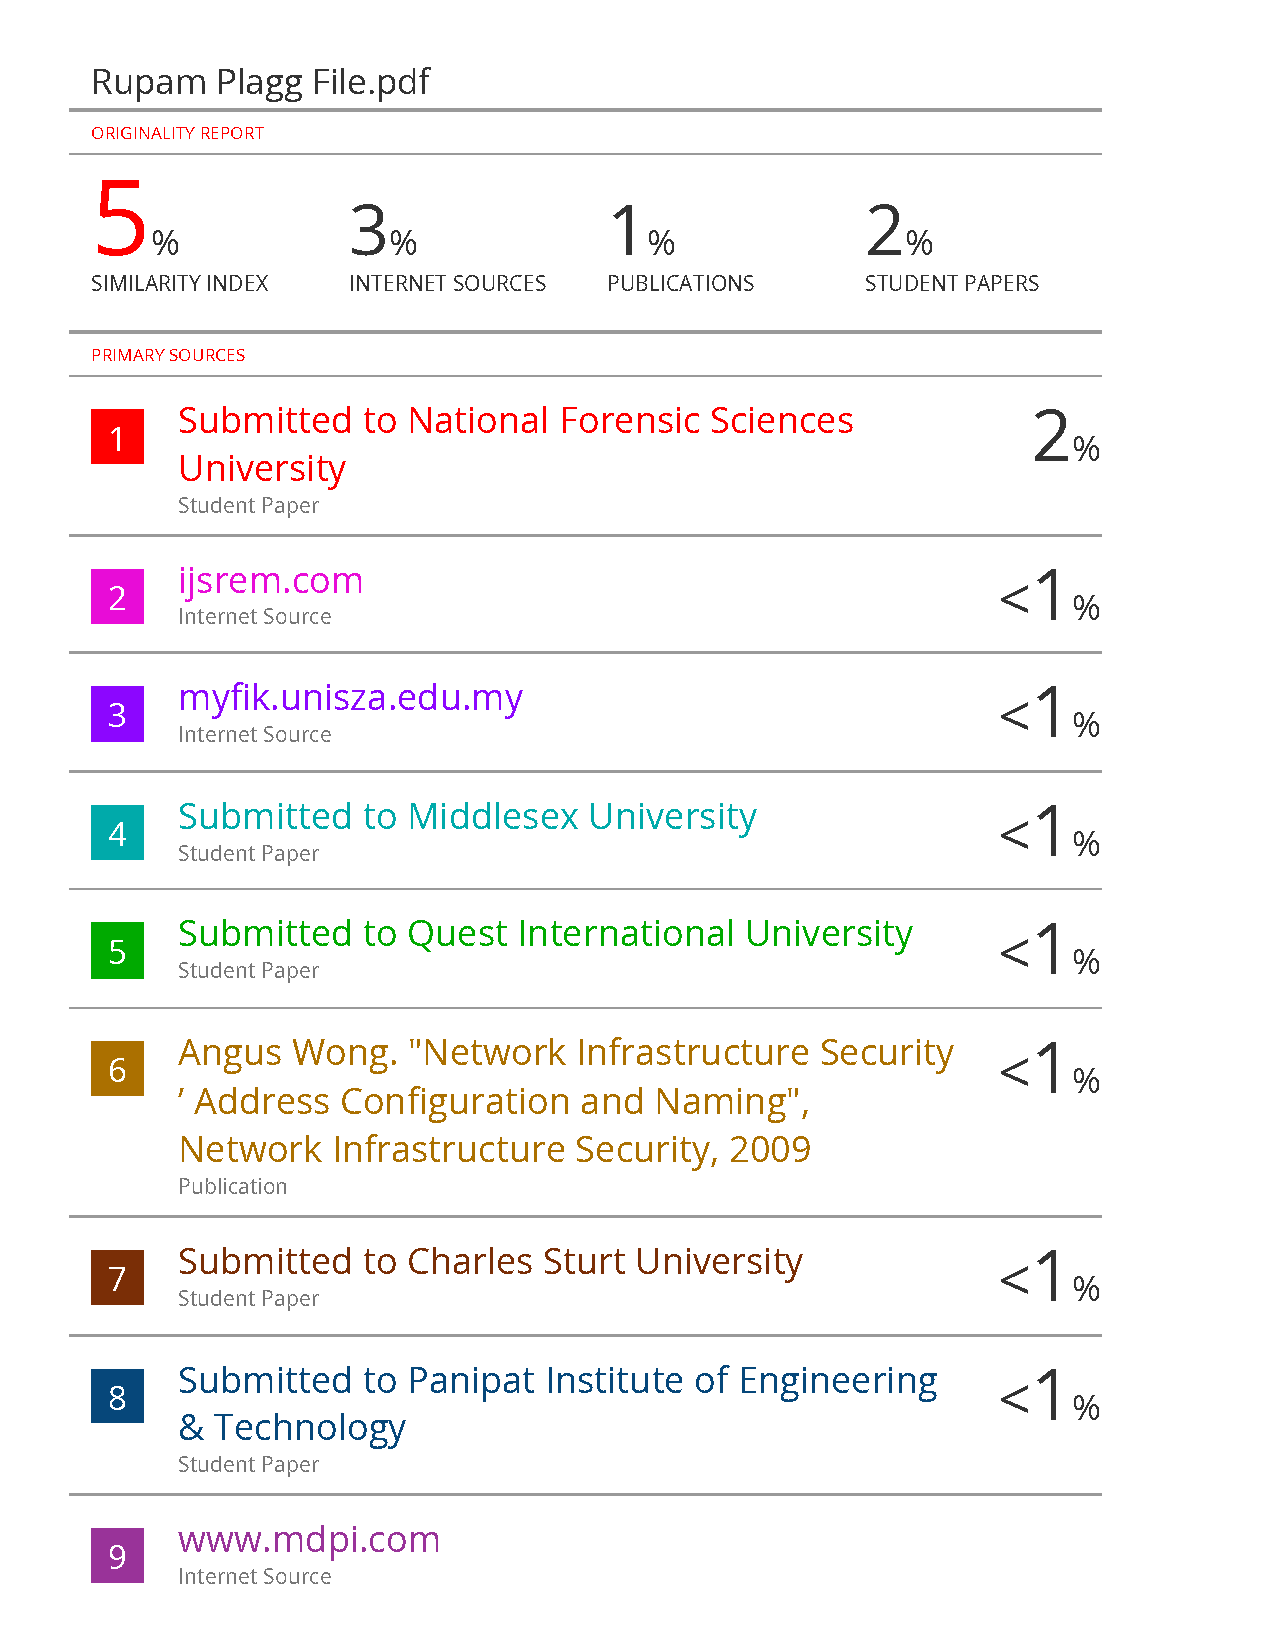
\includepdf[pages=-]{Images/Plagiarism_report.pdf}

\end{document}
